\documentclass[final,5p,times]{elsarticle}
\usepackage{xcolor}
\usepackage{amsmath,amssymb}
\setcounter{secnumdepth}{3}
\usepackage{iftex}
\ifPDFTeX
  \usepackage[T1]{fontenc}
  \usepackage[utf8]{inputenc}
  \usepackage{textcomp}
\else
  \usepackage{unicode-math}
  \defaultfontfeatures{Scale=MatchLowercase}
  \defaultfontfeatures[\rmfamily]{Ligatures=TeX,Scale=1}
  \setmainfont{Times New Roman}
\fi
\usepackage{microtype}
\usepackage{booktabs,array}
\usepackage{longtable}
\usepackage{caption}
\captionsetup[table]{skip=6pt}
\usepackage{calc}
\usepackage{graphicx}
\usepackage{dblfloatfix}
\renewcommand{\dbltopfraction}{0.92}
\renewcommand{\dblfloatpagefraction}{0.88}
\renewcommand{\topfraction}{0.92}
\renewcommand{\bottomfraction}{0.92}
\renewcommand{\textfraction}{0.06}
\setlength{\dbltextfloatsep}{10pt plus 2pt minus 2pt}
\setlength{\floatsep}{8pt plus 2pt minus 2pt}
\setlength{\textfloatsep}{8pt plus 2pt minus 2pt}
\makeatletter
\setlength{\@dblfptop}{0pt}
\setlength{\@dblfpbot}{0pt plus 1fil}
\makeatother
\setlength{\abovedisplayskip}{3.5pt plus 1pt minus 1pt}
\setlength{\belowdisplayskip}{3.5pt plus 1pt minus 2pt}
\setlength{\abovedisplayshortskip}{1.5pt plus 1pt}
\setlength{\belowdisplayshortskip}{1.5pt plus 1pt}
\sloppy
\emergencystretch=3.0em
\tolerance=2000
\hbadness=2000
\journal{Hearing Research}
\usepackage{tikz}
\usetikzlibrary{positioning,arrows.meta}
\usepackage{hyperref}
\hypersetup{
  pdftitle={An effective-circuit model of acute cochlear lateral-wall responses to pharmacological and acoustic perturbations},
  pdfkeywords={Cochlea; Endocochlear potential; Stria vascularis; Potassium recycling; Loop diuretics; Acoustic trauma; Mathematical model},
  hidelinks
}

\title{An effective-circuit model of acute cochlear lateral-wall responses to pharmacological and acoustic perturbations}

\author[uw]{Yi Shen\corref{cor1}}
\cortext[cor1]{Corresponding author at: Department of Speech and Hearing Sciences, University of Washington, 1417 NE 42nd St, Seattle, WA 98105, United States.}
\address[uw]{Department of Speech and Hearing Sciences, University of Washington, 1417 NE 42nd St, Seattle, WA 98105, United States}

\begin{document}
\begin{frontmatter}

\begin{highlights}
\item Integrates four cochlear lateral-wall processes in a 13-state circuit model.
\item One local fit to six studies is an outcome-informed reference, not validation.
\item Local stability and range audits identify limits under severe forcing.
\item Tone comparison underpredicts potassium despite conditional voltage agreement.
\item Scenario grid explores analyst-selected vascular-reserve settings.
\end{highlights}

\begin{abstract}
The cochlear lateral wall maintains the endocochlear potential (EP) and high endolymphatic potassium concentration through coupled electrical, ionic, volume, and metabolic processes. We formulated a reduced 13-state ordinary differential equation model integrating two-battery potassium cycling, intrastrial volume regulation, perfusion--oxygen--adenosine triphosphate energetics, purinergic shunting, and acute acoustic-stress terms. One local, outcome-informed fit estimated nine effective parameters from 178 weighted targets across six published pharmacological and acoustic studies; 71 additional coefficients and the structural closures were fixed. This fit is not independent validation, and the fitted values are not uniquely identified physiological constants. Parameter uncertainty and robustness to alternative residual weights or study inclusion remain unquantified, so the fit is a single exploratory reference realization rather than a robust quantitative prediction. Local Jacobian calculations support local stability at the constructed resting balance, while finite-horizon perturbation simulations show protocol-dependent amplification and do not establish global stability. Severe calibration protocols produce crossings of analyst-selected state-screening ranges, including an ATP-availability cutoff that is not an empirically established physiological limit; endpoint agreement therefore relies in part on trajectories whose physiological plausibility is unresolved. Numerical integration and endpoint fit do not establish physiological validity. An uncalibrated capacity-feedback counterfactual prevents the screened crossings but changes the predicted EP response. In a retrospective, outcome-informed tone comparison, the model underpredicts the reported intrastrial potassium transient by approximately three orders of magnitude; voltage-plateau agreement is obtained only under the selected tone-drive mapping and does not resolve this ionic mismatch. A separate vascular-health grid is an analyst-selected scenario analysis, not empirical evidence of an in-vivo interaction. These results define the scope of the reduced model and identify measurements needed to distinguish voltage-level agreement from the underlying ionic mechanisms.
\end{abstract}

\begin{keyword}
Cochlea \sep Endocochlear potential \sep Stria vascularis \sep Potassium recycling \sep Loop diuretics \sep Acoustic trauma \sep Mathematical model
\end{keyword}

\end{frontmatter}

\section{Introduction}\label{sec:introduction}

\subsection{The endocochlear battery, lateral-wall homeostasis, and auditory sensitivity}\label{sec:intro-battery}

Auditory transduction in the mammalian inner ear is powered by a specialized electrochemical environment within scala media. Unlike standard extracellular fluids, cochlear endolymph maintains a high potassium concentration (\([\mathrm{K}^+]_E \approx 140\text{--}150\,\mathrm{mM}\)), a low sodium concentration (\([\mathrm{Na}^+]_E \approx 1\text{--}2\,\mathrm{mM}\)), and a resting positive direct-current voltage of \(+80\) to \(+100\,\mathrm{mV}\) known as the endocochlear potential (EP) \citep{Davis1958,Wangemann2002}. Paired with the negative intracellular resting potential of cochlear hair cells (\(\approx -70\,\mathrm{mV}\)), the EP establishes a net transmembrane electrical driving force of \(150\text{--}160\,\mathrm{mV}\) across the apical stereociliary bundle. This biological battery drives rapid mechano-electrical transduction (MET) currents in inner and outer hair cells, supporting cochlear amplification, sharp frequency selectivity, and low auditory thresholds across a wide dynamic range.

Maintaining the endocochlear battery places continuous homeostatic demands on the cochlear lateral wall, comprising the stria vascularis and the adjacent spiral ligament. Within the stria vascularis, two potassium diffusion potentials arranged in series across an electrically isolated extracellular microdomain---the intrastrial space (IS)---generate the positive EP \citep{Nin2008,Marcus2002}. Intermediate cells, coupled to basal cells and spiral-ligament fibrocytes into a gap-junctional syncytium, express apical inward-rectifying Kir4.1 (\emph{Kcnj10}) channels facing the narrow intrastrial space. Concurrently, strial marginal cells actively clear potassium from the intrastrial space via basolateral \(\mathrm{Na}^+/\mathrm{K}^+\)-ATPase pumps and bumetanide/furosemide-sensitive \(\mathrm{Na}^+\)-\(\mathrm{K}^+\)-\(2\mathrm{Cl}^-\) cotransporters (NKCC1, \emph{Slc12a2}), keeping intrastrial potassium exceptionally low (\([\mathrm{K}^+]_{\mathrm{IS}} \approx 1.5\text{--}2.0\,\mathrm{mM}\)) relative to the syncytial interior (\(\approx 140\,\mathrm{mM}\)) and secreting potassium back into endolymph through apical KCNQ1/KCNE1 channels \citep{Nin2008,Wangemann2002,Adachi2013}. These coupled electrical, ionic, osmotic, and metabolic processes are not a closed potassium inventory under every perturbation; neither EP nor endolymphatic potassium concentration alone provides a complete diagnostic readout of lateral-wall state.

The principal anatomical compartments and the model's corresponding lumped pathways are summarized in Fig.~\ref{fig:anatomical-overview}.

\begin{figure*}[!t]
  \begin{minipage}[t]{0.81\textwidth}
    \vspace{0pt}
    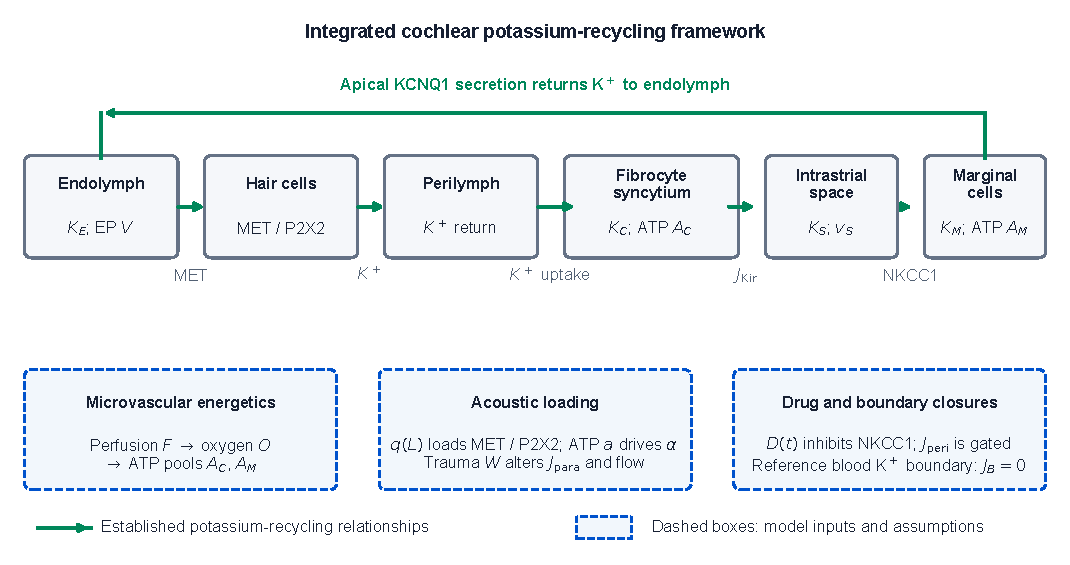
\includegraphics[width=\linewidth]{figures/anatomical-infographic.pdf}
  \end{minipage}\hfill
  \begin{minipage}[t]{0.18\textwidth}
    \vspace{0pt}
    \captionsetup{justification=raggedright,singlelinecheck=false}
    \caption{Anatomical and biophysical overview of the cochlear lateral wall and sensory epithelium (schematic, not to scale). The cross-section identifies the spiral ligament, strial basal, intermediate, and marginal cells, intrastrial space, cochlear scalae, and organ of Corti. Colored arrows and pathway callouts show the effective compartments, fluxes, and furosemide- and noise-associated mechanisms represented in the 13-state model; these are model abstractions rather than cell-resolved anatomical measurements.}
    \label{fig:anatomical-overview}
  \end{minipage}
\end{figure*}

Clinically and translationally, lateral-wall homeostasis is a primary determinant of auditory vulnerability across the lifespan. In Schuknecht's classical histopathological framework and modern physiological phenotyping, strial or metabolic presbycusis represents a major subtype of age-related hearing loss characterized by lateral-wall atrophy, microvascular rarefaction, and reduced EP driving intact sensory hair bundles \citep{Schuknecht1974,Ohlemiller2006,Ohlemiller2009,Vaden2022}. However, chronic histological correlations in aging animals have shown that substantial strial cellular or capillary loss can occur with only modest reductions in quiet resting EP until functional reserve is exhausted \citep{Ohlemiller2006,Ohlemiller2009}. Understanding how microvascular delivery, cellular energetics, ion transport, and sensory loading interact therefore requires examining the lateral wall not only at rest, but dynamically under acute pharmacological and acoustic stress.

\subsection{Previous modeling efforts and the rationale for an integrative dynamical framework}\label{sec:intro-prior-models}

Mathematical and electrical modeling has played a central role in cochlear physiology since the foundational resistance-network formulation of \citet{Davis1958}. In the modern era, the experimental microelectrode demonstrations of \citet{Nin2008} and the quantitative six-compartment circulation-current model of \citet{Nin2012} (further synthesized in \citealt{NinHibino2016}) established the biophysical basis of mammalian EP electrogenesis. Specifically, \citet{Nin2012} integrated membrane channel conductances, active pump and NKCC1 cotransporter fluxes, and compartmental ion balances to reproduce time-domain electrochemical trajectories during anoxia and vascular perfusion of ouabain or bumetanide, demonstrating how circulation current and intrastrial potassium accumulation govern the rise and collapse of the intrastrial potential (ISP) and EP. Related modeling work has addressed cochlear fluid volume regulation and longitudinal solute dispersion \citep{Salt2001}.

The present work builds directly upon these foundational modeling efforts. Rather than proposing novel cellular mechanisms or claiming channel-level superiority over the detailed membrane-transport formulation of \citet{Nin2012}, this study develops an effective-circuit framework for diagnostic analysis. Previous experimental work has largely examined four interacting physiological domains separately. Studies of strial electrogenesis and loop-diuretic pharmacodynamics show that furosemide or bumetanide transiently inhibits marginal-cell potassium uptake, reduces EP to negative values (\(-30\) to \(-40\,\mathrm{mV}\)), increases cochlear partition resistance, and depletes endolymphatic potassium over 60--120 min \citep{Bosher1979,PikeBosher1980,AsakumaSnow1980,RybakMorizono1982}. Related work on intrastrial volume regulation describes solute retention and reversible extracellular edema when marginal-cell clearance is impaired \citep{SantiDuvall1979,PikeBosher1980,Salt2001}. In the vascular and metabolic domain, increased demand can trigger lactate- and nitric-oxide-mediated capillary dilation \citep{Dai2011}, whereas intense noise or ischemia can induce vasoconstriction, hypoxia, and ATP depletion \citep{PrazmaPecorak1975,Kusakari1978,Nuttall1999,Shi2016,Hou2020}. Finally, studies of purinergic acoustic adaptation show that sound-evoked endolymphatic ATP release gates apical P2X2 channels, shunting the cochlear partition and attenuating hair-cell transducer drive; at higher intensities, EP depression and paracellular barrier leakage have also been reported \citep{Munoz2001,Telang2010,Housley2013,SaltKonishi1979,Wang1990,Wang1992,Ohlemiller2018}.

This study combines reduced representations of these four physiological processes in a computationally tractable 13-state effective-circuit ordinary differential equation (ODE) model. Joint fitting across pharmacological and acoustic observations provides an outcome-informed consistency check on this chosen structure; it does not demonstrate that the model is uniquely mechanistic or prospectively predictive.

\subsection{Rationale for integrating pharmacological and acoustic perturbations}\label{sec:intro-motivation}

A recurring challenge in biological modeling is underdetermination: a model tuned to a single voltage trace can closely follow the observed trajectory through compensating parameter adjustments that obscure an incorrect underlying ionic or energetic mechanism. We therefore compare acute loop-diuretic administration and acoustic overstimulation as a diagnostic stress test of the selected effective formulation. Joint fitting across these perturbations can expose endpoint tensions, but does not by itself prevent parameter compensation, establish robustness, or demonstrate predictive validity.

First, furosemide and intense sound interrogate opposite ends of the cochlear potassium-recycling loop. Loop diuretics primarily target the strial source---suppressing marginal-cell basolateral uptake and source conductance while reducing transport ATP consumption---whereas acoustic stimulation primarily modulates the sensory sink and protective shunts---increasing hair-cell MET conductance, recruiting ATP-gated P2X2 channels, and inducing mechanical adaptation or trauma-associated vascular and barrier stress. A shared parameter set provides a common descriptive comparison across these responses, but does not prevent sensory-load parameters from compensating for strial-source errors or vice versa.

Second, considering multiple experimental endpoints---including EP time courses, endolymphatic potassium changes (\(\Delta K_E\)), cochlear partition resistance ratios (\(R/R_0\)), and ISP/EP voltage recordings---helps expose limitations that voltage-only fitting could conceal. The Zhang et al. (2021) voltage group means and representative intrastrial potassium trace were acquired in sequential electrode-position recordings, not as simultaneous paired measurements. In this retrospective comparison, the model matches the sustained voltage plateaus while underpredicting the reported potassium transient by approximately three orders of magnitude. This comparison illustrates how the effective circuit's voltage fit can coexist with a mismatch in the modeled ionic response; it does not identify the in-vivo mechanism.

Third, an acute effective-circuit framework may motivate future tests of multi-hit and chronic cochlear pathologies, but the present model does not directly represent or validate drug--noise interactions. Recent experimental studies have reported such interactions \citep{Su2026} and long-term vascular consequences of acoustic trauma \citep{Hou2020}. The analyst-selected vascular and trauma-susceptibility grid below is a scenario analysis that compares resting EP deficits with simulated acute responses; it does not establish latent vulnerability or an in-vivo interaction.

\subsection{Overview of the manuscript organization and scope boundaries}\label{sec:intro-organization}

The manuscript first presents the mathematical formulation and its biophysical rationale, including the compartmental architecture and simplifying closures (Section~\ref{sec:formulation}; Fig.~\ref{fig:anatomical-overview}; Tables~\ref{tab:model-states} and~\ref{tab:model-parameters}). It then describes joint calibration across six anchoring studies, freezes the parameter vector, and evaluates local residual geometry and protocol-exclusion sensitivity (Section~\ref{sec:calibration}; Table~\ref{tab:fitting-studies}; Fig.~\ref{fig:tier1}). Stability, perturbation, and flux-budget analyses follow (Section~\ref{sec:stability}; Figs.~\ref{fig:diagnostics} and~\ref{fig:scenario-states}), followed by retrospective benchmarks against tone-evoked ISP/EP recordings and microvascular injury observations (Section~\ref{sec:benchmarks}; Figs.~\ref{fig:zhang} and~\ref{fig:hou}). The discussion considers alignment with broader lateral-wall physiology (Section~\ref{sec:alignment}), methodological and structural limitations (Section~\ref{sec:limitations}), and implications for experimental design and future multiscale modeling (Section~\ref{sec:future}).

\paragraph*{Scope and epistemic boundaries}
Throughout this study, we maintain a strict distinction between mechanistic unification and unvalidated extrapolation. The model is an acute, single-turn lumped representation with explicit effective closures. Both the six-study calibration and the retrospective benchmark transfers are outcome-informed mechanistic stress tests rather than untouched out-of-sample clinical predictions. Finite numerical diagnostics establish local rest attraction and bounded trajectory behavior over the tested horizons but do not constitute analytical proofs of global stability or parameter uniqueness. Spatial base-to-apex gradients, weeks-long cellular remodeling, chronological aging, and cellular regeneration lie outside the modeled equations and are addressed strictly as directions for future multiscale extensions.

\section{Mathematical formulation and biophysical justifications}\label{sec:formulation}

\subsection{System architecture and 13-state compartmental representation}\label{sec:formulation-states}

The cochlear lateral wall and scala media are formulated as a coupled 13-state lumped dynamical system governed by the first-order ordinary differential equation vector
\begin{equation}
  \frac{d\mathbf{x}}{dt} = f\bigl(\mathbf{x}(t), \mathbf{u}(t); \boldsymbol{\theta}\bigr),
  \label{eq:ode}
\end{equation}
where \(\mathbf{x}(t) \in \mathbb{R}^{13}\) denotes the state vector, \(\mathbf{u}(t)\) represents exogenous pharmacological and acoustic protocol inputs, and \(\boldsymbol{\theta}\) comprises the model parameters. In solver order, the 13 differential states are: relative strial capillary perfusion \(F\), lateral-wall dissolved oxygen availability \(O\), syncytial and marginal-cell ATP-availability proxies \(A_C\) and \(A_M\), normalized intrastrial extracellular volume \(v_S\), syncytial potassium concentration \(K_C\), intrastrial potassium concentration \(K_S\), marginal-cell potassium concentration \(K_M\), the endocochlear potential \(V\), bulk endolymphatic ATP concentration \(a\) (Latin \(a\)), total modeled potassium inventory \(N_K\), a mechanotransducer adaptation proxy \(\alpha\) (Greek \(\alpha\)), and a reversible acute acoustic-trauma proxy \(W\).

\paragraph*{Architecture guide}
The anatomical context and mapping from cochlear structures to the model's lumped compartments are shown in Fig.~\ref{fig:anatomical-overview}. The 13 states are grouped into four functional subsystems (Table~\ref{tab:model-states}). The microvascular and energetic subsystem comprises perfusion \(F\), oxygen availability \(O\), and ATP-availability proxies \(A_C\) and \(A_M\); perfusion supplies oxygen, oxidative metabolism replenishes the energy stores, and ATP depletion promotes vasodilation in competition with trauma-induced vasoconstriction. The volume and potassium-recycling subsystem comprises \(v_S, K_C, K_S, K_M,\) and \(N_K\). The syncytial potassium state \(K_C\) is a lumped intracellular pool, not a cell-specific measurement. Potassium cycles from endolymph through hair-cell MET and P2X2 channels into perilymph and the lateral-wall syncytium, then across Kir4.1 channels into the intrastrial space, through marginal cells, and back into endolymph. Intrastrial potassium accumulation drives osmotic water influx, while \(N_K\) tracks total potassium mass. The electrogenic circuit subsystem is represented by EP \(V\): gradients across the intermediate-cell and marginal-cell membranes establish two diffusion batteries in series, which charge EP and ISP against the current drain of MET and P2X2 conductances. The purinergic, adaptation, and trauma subsystem comprises endolymphatic ATP \(a\), transducer adaptation \(\alpha\), and acute trauma \(W\). Sound-evoked ATP activates the apical P2X2 shunt and recruits adaptation, whereas intense overstimulation induces trauma-associated paracellular potassium leakage, residual transducer load, and vasoconstriction.

Rather than introducing redundant differential equations for dependent quantities, endolymph volume \(v_E\) and endolymphatic potassium concentration \(K_E\) are defined algebraically from the volume balance and current modeled potassium inventory:
\begin{equation}
  \begin{aligned}
    v_E &= 1 + v_{S,0} - v_S,\\
    K_E &= \frac{N_K - \phi_C K_C - v_S K_S - \phi_M K_M}{v_E}.
  \end{aligned}
  \label{eq:endolymph}
\end{equation}
Here, all compartment volumes are normalized to the resting endolymph volume (\(V_{E,0} = 1\), so \(v_{E,0} = 1\)), whereas \(\phi_C = 0.40\) and \(\phi_M = 0.042\) denote the fixed effective volume ratios of the syncytial and marginal-cell compartments relative to \(V_{E,0}\) (contextualized by guinea-pig strial morphometry; \citealt{SantiDuvall1979,Salt2001}). At the reference resting state, \(F_0 = 1\), \(O_0 = 0.07\,\mathrm{mM}\), \(A_{C,0} = A_{M,0} = 1\), \(v_{S,0} = 0.035\), \(K_{C,0} = 140\,\mathrm{mM}\), \(K_{S,0} = 1.5\,\mathrm{mM}\), \(K_{M,0} = 145\,\mathrm{mM}\), \(V_0 = 80\,\mathrm{mV}\), \(a_0 = 0.0074\,\mu\mathrm{M}\) (\(7.4\,\mathrm{nM}\)), \(N_{K,0} = 212.1425\,\mathrm{mM}\,V_{E,0}\) (yielding \(K_{E,0} = 150\,\mathrm{mM}\)), and \(\alpha_0 = W_0 = 0\).

% Generated by build_parameter_table.py; do not hand-edit.
\begin{table*}[!t]
\caption{All 13 differential states of the frozen reference model, in solver order. Baselines are initial conditions, not fitted population means or a certified exact equilibrium. \(V_{E,0}\) denotes resting endolymph volume; relative ATP is a normalized availability proxy.}\label{tab:model-states}
\centering\small
\setlength{\tabcolsep}{4pt}\renewcommand{\arraystretch}{1.13}
\begin{tabular}{@{}>{\raggedright\arraybackslash}p{1.1cm}>{\raggedright\arraybackslash}p{3.6cm}r>{\raggedright\arraybackslash}p{2.1cm}>{\raggedright\arraybackslash}p{7.4cm}@{}}
\toprule \textbf{Symbol} & \textbf{State} & \textbf{Initial value} & \textbf{Units} & \textbf{Interpretation} \\ \midrule
\(F\) & Relative strial perfusion & 1 & relative flow & Lumped delivery state; not a local vessel-flow measurement. \\
\(O\) & Tissue oxygen availability & 0.07 & mM & Effective dissolved-oxygen pool. \\
\(A_C\) & Syncytial ATP availability & 1 & relative ATP & Normalized energetic proxy, not measured ATP concentration. \\
\(A_M\) & Marginal-cell ATP availability & 1 & relative ATP & Normalized energetic proxy, not measured ATP concentration. \\
\(v_S\) & Intrastrial extracellular volume & 0.035 & \(V_{E,0}\) & Effective cleft volume relative to resting endolymph. \\
\(K_C\) & Syncytial potassium & 140 & mM & Lumped intracellular K pool. \\
\(K_S\) & Intrastrial potassium & 1.5 & mM & Extracellular K pool. \\
\(K_M\) & Marginal-cell potassium & 145 & mM & Lumped intracellular K pool. \\
\(V\) & Endocochlear potential & 80 & mV & Dynamic circuit voltage. \\
\(a\) & Bulk endolymph ATP & 0.0074 & \(\mu\mathrm{M}\) & Bulk ATP; receptor-level ATP is derived algebraically. \\
\(N_K\) & Total modeled potassium inventory & 212.1425 & mM \(V_{E,0}\) & Inventory, not a compartment concentration; conserved for sealed boundaries. \\
\(\alpha\) & Transducer-adaptation proxy & 0 & dimensionless & Phenomenological attenuation state, nominal domain 0--1. \\
\(W\) & Acoustic-trauma proxy & 0 & dimensionless & Reversible acute-injury state, nominal domain 0--1; not chronic remodeling. \\
\bottomrule\end{tabular}
\par\smallskip\raggedright\footnotesize Endolymph volume \(v_E\), endolymph K \(K_E\), intrastrial potential (ISP), and receptor-level ATP are algebraic observables, not additional states. Drug drive, sound multiplier and ATP delivery are exogenous inputs; the furosemide-protocol flag selects a boundary condition. Inventory changes only through explicit boundary exchange.
\end{table*}


\subsection{Two-battery potassium electrogenesis, sensory loading, and effective ion fluxes}\label{sec:formulation-electrogenesis}

Following the two-battery paradigm of \citet{Nin2008,Nin2012}, the primary electromotive forces within the stria vascularis are the potassium Nernst diffusion potentials across the syncytial--intrastrial interface (\(E_{CS}\), mediated by intermediate-cell Kir4.1 channels) and the marginal--endolymphatic interface (\(E_{ME}\), mediated by apical KCNQ1/KCNE1 channels):
\begin{equation}
  \begin{aligned}
    E_{CS} &= V_T \ln\left(\frac{K_C}{K_S}\right),\\
    E_{ME} &= V_T \ln\left(\frac{K_M}{K_E}\right),
  \end{aligned}
  \label{eq:nernst}
\end{equation}
where \(V_T = 26.7\,\mathrm{mV}\) is the thermal voltage \(RT/F\) at mammalian body temperature (\(\approx 310\,\mathrm{K}\)). At rest, the steep gradient between syncytial potassium (\(140\,\mathrm{mM}\)) and the actively depleted intrastrial space (\(1.5\,\mathrm{mM}\)) yields a large positive battery \(E_{CS,0} = +121.1\,\mathrm{mV}\), whereas the near-equal potassium concentrations in marginal cells (\(145\,\mathrm{mM}\)) and endolymph (\(150\,\mathrm{mM}\)) yield a near-zero apical battery \(E_{ME,0} = -0.91\,\mathrm{mV}\).

When acoustic stimulation elevates bulk endolymphatic ATP \(a(t)\) above its resting baseline \(a_0\), the local ATP concentration within the subtectorial hair-bundle cleft is amplified by a microdomain factor \(c_a = 30\), yielding \(a_r = a_0 + c_a\max(0, a - a_0)\), which gates an apical purinergic P2X2 shunt conductance \citep{Munoz2001,Housley2013}:
\begin{equation}
  g_P(a_r) = g_{P,\max}\frac{a_r^{n_P}}{a_r^{n_P} + K_P^{n_P}}.
  \label{eq:gp}
\end{equation}
Let \(q(t) \ge 1\) denote the acoustic drive multiplier, \(e(t) = \max(0, q(t) - 1)\) the excess acoustic drive, and \(h_D(t) \in (0,1]\) the fractional availability of furosemide-sensitive strial transport. The effective hair-cell mechanotransduction load factor \(m(t)\) and strial source conductance \(g_S(t)\) are expressed as
\begin{align}
  m &= 1 - r_\alpha \alpha(1 - W) + e(1 - e_\alpha \alpha) + 0.35W, \label{eq:met-factor}\\
  g_S &= g_{S,0}\left[1 - \ell_D(1 - h_D)\right]. \label{eq:gs}
\end{align}
In Eq.~(\ref{eq:met-factor}), transducer adaptation \(\alpha\) attenuates both the resting MET opening probability (weighted by \(r_\alpha\)) and the sound-evoked drive \(e\) (weighted by \(e_\alpha\)), whereas acute trauma \(W\) diminishes resting adaptation control and introduces a persistent load component (\(0.35W\)).

Let \(\bar{A} = (A_C + A_M)/2\) denote the mean lateral-wall ATP-availability proxy. The effective strial source voltage \(V_S\), total scala media circulation current \(I_{\mathrm{circ}}\), and dynamic EP rate equation are given by
\begin{align}
  V_S &= f_K E_{CS} + E_{ME} + V_{\mathrm{pump}}\bar{A} - V_{\mathrm{off}}, \label{eq:vs}\\
  I_{\mathrm{circ}} &= g_{\mathrm{MET}} m \max(0, V - V_{\mathrm{MET}}) + g_P(a_r)(V - V_P), \label{eq:icirc}\\
  \frac{dV}{dt} &= \frac{g_S(V_S - V) - I_{\mathrm{circ}}}{C_V}. \label{eq:voltage}
\end{align}
Simultaneously, the intrastrial potential (\(V_{\mathrm{ISP}}\)) recorded by a microelectrode positioned inside the intrastrial space is modeled as an algebraic observation of the intermediate-cell diffusion battery under the resistive drop of the same circulation current:
\begin{equation}
  V_{\mathrm{ISP}} = f_K E_{CS} - V_{\mathrm{ISP,off}} - R_C I_{\mathrm{circ}}.
  \label{eq:isp}
\end{equation}

\paragraph*{Biophysical justification and effective-circuit qualifications}
Equations~(\ref{eq:gs})--(\ref{eq:isp}) represent a reduced effective circuit designed to bridge heterogeneous \emph{in vivo} datasets rather than a channel-by-channel replica of \citet{Nin2012}. Three specific simplifications warrant explicit justification. First, in Eq.~(\ref{eq:vs}), the term \(V_{\mathrm{pump}}\bar{A}\) (with \(V_{\mathrm{pump}} = 15\,\mathrm{mV}\)) and static offset \(V_{\mathrm{off}} = 10.16\,\mathrm{mV}\) provide a phenomenological energetic coupling that links acute ATP depletion to source voltage alongside indirect ion-gradient changes; it is not a first-principles derivation of \(\mathrm{Na}^+/\mathrm{K}^+\)-ATPase electrogenicity, and the equal weighting of \(A_C\) and \(A_M\) is an inherited symmetry assumption. Second, when furosemide inhibits marginal-cell uptake (\(h_D \to 0\)), Eq.~(\ref{eq:gs}) reduces the effective strial source conductance \(g_S\) by the fraction \(\ell_D\). Although biological NKCC1 cotransporters are electroneutral, severe loop-diuretic block collapses the strial source path and roughly doubles total cochlear partition resistance \citep{AsakumaSnow1980}, allowing the negative hair-cell diffusion potential (\(V_{\mathrm{MET}} = -70\,\mathrm{mV}\) in Eq.~\ref{eq:icirc}) to pull scala media EP to negative nadirs between \(-30\) and \(-40\,\mathrm{mV}\) \citep{Bosher1979,PikeBosher1980}. Thus, \(\ell_D\) represents a lumped circuit conductance surrogate rather than the molecular fraction of inhibited NKCC1 proteins.

To couple ion transport to cellular energetics and substrate availability, the normalized active transport workloads in the syncytium (\(U_C\)) and marginal cells (\(U_M\)) follow saturating Michaelis--Menten kinetics normalized to unity at rest:
\begin{align}
  U_C &= \frac{A_C}{K_{m,C} + A_C}\frac{K_{m,C} + A_0}{A_0}\frac{K_E}{K_{E,0}}, \label{eq:uc}\\
  U_M &= \frac{A_M}{K_{m,M} + A_M}\frac{K_{m,M} + A_0}{A_0}\frac{K_S}{K_{m,K} + K_S}\frac{K_{m,K} + K_{S,0}}{K_{S,0}}. \label{eq:um}
\end{align}
In Eq.~(\ref{eq:um}), marginal-cell uptake \(U_M\) is dually regulated by marginal ATP availability \(A_M\) (\(K_{m,M} = 0.45\)) and intrastrial potassium substrate \(K_S\) (\(K_{m,K} = 4.0\,\mathrm{mM}\)), reflecting the high sensitivity of basolateral NKCC1 and \(\mathrm{Na}^+/\mathrm{K}^+\)-ATPase clearance to rising intrastrial potassium \citep{Nin2008,NinHibino2016}.

The resulting unidirectional and net potassium inventory fluxes (in units of \(\mathrm{mM}\,V_{E,0}\,\mathrm{min}^{-1}\), where \(q_K = 2.8\,\mathrm{mM}\,V_{E,0}\,\mathrm{min}^{-1}\) is the balanced resting turnover rate; \citealt{Konishi1978,Nin2012}) are given by
\begin{align}
  J_{\mathrm{Kir}} &= \frac{f_K q_K (K_C - K_S)}{K_{C,0} - K_{S,0}}\left|\frac{E_{CS}}{E_{CS,0}}\right|, \label{eq:jkir}\\
  J_U &= q_K h_D U_M, \label{eq:ju}\\
  J_A &= q_K \frac{K_M}{K_{M,0}}, \label{eq:ja}\\
  J_{\mathrm{MET}} &= q_K m \frac{\max(0, V - V_{\mathrm{MET}})}{V_0 - V_{\mathrm{MET}}}\frac{K_E}{K_{E,0}}, \label{eq:jmet}\\
  J_{\mathrm{P2X}} &= q_K \frac{g_P(a_r) - g_{P,0}}{g_{\mathrm{MET}}}\frac{V - V_P}{V_0 - V_{\mathrm{MET}}}\frac{K_E}{K_{E,0}}, \label{eq:jp2x}\\
  J_{\mathrm{para}} &= (\ell_0 + \ell_W W)(K_C - K_S), \label{eq:jpara}\\
  J_B &= b_K(K_{\mathrm{plasma}} - K_S). \label{eq:jb}
\end{align}
Here, \(J_{\mathrm{Kir}}\) represents potassium efflux from the syncytium into the intrastrial space scaled by the normalized chemical gradient and diffusion potential (a concentration-gradient surrogate rather than a voltage-rectified Hodgkin--Huxley channel law); \(J_U\) is furosemide-sensitive basolateral marginal uptake; \(J_A\) is apical marginal potassium secretion into endolymph; \(J_{\mathrm{MET}}\) and \(J_{\mathrm{P2X}}\) represent potassium clearance from endolymph through hair-cell MET channels and ATP-gated P2X2 channels (normalized relative to the resting MET conductance \(g_{\mathrm{MET}}\) and driving force \(V_0 - V_{\mathrm{MET}}\)); \(J_{\mathrm{para}}\) represents paracellular syncytial--intrastrial leakage across tight junctions (with \(\ell_0 = 0\) at rest due to intact Claudin-11 barriers and \(\ell_W W\) recruited during acoustic trauma); and \(J_B\) represents direct trans-endothelial potassium exchange across the intrastrial fluid--blood barrier (\(b_K = 0\) in the intact reference state; \citealt{Shi2016}).

During severe loop-diuretic blockade, chinchilla and guinea-pig recordings demonstrate a substantial net reduction in endolymphatic potassium concentration (\(-15.7\) to \(-32.5\,\mathrm{mM}\); \citealt{RybakMorizono1982}) that cannot be accommodated solely by redistributing potassium into the minuscule intrastrial volume (\(v_{S,0} = 0.035\)). To capture this net clearance into the large perilymphatic reservoir during diuretic challenge while setting the external perilymphatic flux to zero during acoustic protocols, the boundary flux is formulated as
\begin{equation}
  J_{\mathrm{peri}} = \mathbf{1}_{\mathrm{drug}}\Bigl[\ell_D^K (K_E - K_{\mathrm{plasma}})(1 - h_D) + r_D^K (K_E - K_{E,0}) h_D\Bigr],
  \label{eq:jperi}
\end{equation}
where \(\mathbf{1}_{\mathrm{drug}} \in \{0,1\}\) is the pharmacological protocol indicator, \(\ell_D^K\) governs potassium loss down the endolymph--perilymph gradient when NKCC1 is inhibited, and \(r_D^K\) governs post-washout inventory restoration. As analyzed in Section~\ref{sec:stability-counterfactuals}, we treat this protocol-gated boundary law as an explicit, falsifiable closure hypothesis and evaluate counterfactuals in which the boundary is either sealed during drug exposure or opened across all protocols.

Combining these fluxes yields differential balance equations for intrastrial extracellular volume \(v_S\), compartmental potassium concentrations \(K_C, K_S, K_M\), and total potassium inventory \(N_K\):
\begin{align}
  \frac{dv_S}{dt} &= 2P_w \sigma_K (K_S - K_{S,0}) - k_v (v_S - v_{S,0})\left[1 + \left(\frac{v_S - v_{S,0}}{v_{\mathrm{span}}}\right)^2\right], \label{eq:dvs}\\
  \frac{dK_C}{dt} &= \frac{J_{\mathrm{MET}} + J_{\mathrm{P2X}} - J_{\mathrm{Kir}} - J_{\mathrm{para}}}{\phi_C}, \label{eq:dkc}\\
  \frac{dK_S}{dt} &= \frac{J_{\mathrm{Kir}} + J_{\mathrm{para}} - J_U + J_B}{v_S} - \frac{K_S}{v_S}\frac{dv_S}{dt}, \label{eq:dks}\\
  \frac{dK_M}{dt} &= \frac{J_U - J_A}{\phi_M}, \label{eq:dkm}\\
  \frac{dN_K}{dt} &= J_B - J_{\mathrm{peri}}. \label{eq:dnk}
\end{align}
Equation~(\ref{eq:dvs}) captures osmotic swelling of the intrastrial space driven by potassium salt accumulation (\(2P_w \sigma_K [K_S - K_{S,0}]\)) balanced by nonlinear viscoelastic tissue restoration \citep{SantiDuvall1979,PikeBosher1980}, while the second term in Eq.~(\ref{eq:dks}) rigorously accounts for concentration dilution/concentration due to dynamic volume changes \(dv_S/dt\).

\subsection{Microvascular perfusion, oxygen extraction, and compartmental ATP energetics}\label{sec:formulation-energetics}

The stria vascularis exhibits one of the highest metabolic rates in the mammalian body and is acutely vulnerable to reductions in capillary perfusion or oxygen tension \citep{PrazmaPecorak1975,Kusakari1978,Nuttall1999}. Using the mean lateral-wall ATP-availability proxy \(\bar{A}\), relative strial capillary perfusion \(F(t)\) relaxes with time constant \(\tau_F = 1.5\,\mathrm{min}\) toward a smooth positive target \(F_\infty\) that balances metabolic vasodilation against trauma-associated vasoconstriction:
\begin{align}
  F^* &= F_0\left[1 + \rho\frac{A_0 - \bar{A}}{A_0}\right](1 - \rho_W W), \label{eq:fstar}\\
  F_\infty &= F_{\min} + \frac{(F^* - F_{\min}) + \sqrt{(F^* - F_{\min})^2 + \epsilon_F^2}}{2}, \label{eq:flow-target}\\
  \frac{dF}{dt} &= \frac{F_\infty - F}{\tau_F}. \label{eq:df}
\end{align}
In Eq.~(\ref{eq:fstar}), an energetic deficit (\(\bar{A} < A_0\)) recruits compensatory vasodilation with gain \(\rho = 0.55\) (representing metabolic autoregulation via lactate and nitric oxide signaling in spiral-ligament type V fibrocytes and strial pericytes; \citealt{Dai2011}), whereas acoustic trauma \(W\) induces capillary constriction with weight \(\rho_W\) \citep{Nuttall1999,Hou2020}. Equation~(\ref{eq:flow-target}) enforces a smooth lower perfusion floor \(F_{\min} = 0.12\) with regularization width \(\epsilon_F = 0.01\) to preserve continuous differentiability.

Capillary oxygen extraction \(X_F\), oxidative phosphorylation capacity \(O_x\), whole-tissue metabolic demand \(M\), and the lateral-wall dissolved oxygen balance \(dO/dt\) are modeled as
\begin{align}
  F_s &= \max(F, 10^{-4}), \label{eq:fs}\\
  X_F &= \frac{F_s\left[1 - \exp(-p_O / F_s)\right]}{1 - \exp(-1)}, \label{eq:xf}\\
  O_x &= \frac{O}{K_{m,O} + O}\frac{K_{m,O} + O_0}{O_0}, \label{eq:ox}\\
  M &= M_0 O_x \max\bigl[0.2, 1 + \eta(A_0 - \bar{A})\bigr], \label{eq:met-demand}\\
  \frac{dO}{dt} &= p_F X_F(O_a - O) - \nu_O s_O M. \label{eq:do}
\end{align}
Equation~(\ref{eq:xf}) implements the classical Renkin--Crone capillary extraction relation normalized to unity at resting flow (\(F_s = 1, p_O = 1\)), capturing how reduced perfusion increases fractional transit-time extraction while reducing total oxygen delivery \(F_s[1 - \exp(-p_O/F_s)]\).

Finally, the syncytial and marginal-cell ATP availability proxies \(A_C\) and \(A_M\) evolve according to the balance between oxygen-dependent synthesis and compartmental consumption (\(C_C\) and \(C_M\)):
\begin{align}
  C_C &= (1 - \eta_C)A_C + \eta_C U_C, \label{eq:cc}\\
  C_M &= (1 - \eta_M)A_M + \eta_M h_D U_M, \label{eq:cm}\\
  \frac{dA_C}{dt} &= \frac{2O_x / (1 + A_C / A_0) - C_C}{\tau_C}, \label{eq:dac}\\
  \frac{dA_M}{dt} &= \frac{2O_x / (1 + A_M / A_0) - C_M}{\tau_M}. \label{eq:dam}
\end{align}
Here, \(\eta_C = 0.65\) and \(\eta_M = 0.78\) partition cellular ATP turnover between basal housekeeping demand (\((1 - \eta_i)A_i\)) and active ion-transport workload (\(\eta_C U_C\) and \(\eta_M h_D U_M\)). At the resting baseline (\(O_x = 1, U_C = U_M = 1, h_D = 1\)), synthesis \(2O_x/(1 + A_i/A_0) = 1\) exactly balances consumption \(C_i = 1\).

\subsection{Purinergic P2X2 signaling, transducer adaptation, and acute acoustic trauma}\label{sec:formulation-purinergic}

The fourth subsystem couples acoustic drive to endolymphatic purinergic signaling, hair-cell transducer adaptation, and reversible acoustic trauma. Bulk endolymphatic ATP concentration \(a(t)\) evolves through basal release, sound-evoked secretion from marginal and supporting cells (attenuated by adaptation \(\alpha\)), exogenous infusion \(I_a(t)\) (zero in all non-injection protocols), ectonucleotidase clearance \(k_a a\), and endolymphatic volume change:
\begin{equation}
  \frac{da}{dt} = \frac{k_a a_0 v_E + r_a(1 - 0.55\alpha)e + I_a}{v_E} - k_a a + \frac{a}{v_E}\frac{dv_S}{dt}.
  \label{eq:atp-endo}
\end{equation}

Transducer adaptation \(\alpha(t) \in [0,1]\) integrates a direct mechanical sound-drive recruitment term \(H_\alpha(e)\) with a purinergic P2X2 conductance recruitment term (weighted by \(r_P = 0.78\); \citealt{Housley2013}), while acute acoustic trauma \(W(t) \in [0,1]\) accumulates above a steep high-intensity threshold \(H_W(e)\) and decays exponentially during post-exposure recovery with time constant \(\tau_R = 95\,\mathrm{min}\):
\begin{align}
  H_\alpha(e) &= \frac{e^{n_\alpha}}{e^{n_\alpha} + K_\alpha^{n_\alpha}}, \label{eq:halpha}\\
  H_W(e) &= \frac{e^{n_W}}{e^{n_W} + K_W^{n_W}}, \label{eq:hw}\\
  P_\alpha &= (1 - r_P)H_\alpha(e) + r_P\frac{\Delta g}{K_{\Delta g} + \Delta g}, \label{eq:palpha}\\
  \frac{d\alpha}{dt} &= r_\alpha^{\mathrm{rate}} P_\alpha(1 - \alpha) - \frac{\alpha}{\tau_\alpha}, \label{eq:dalpha}\\
  \frac{dW}{dt} &= \frac{H_W(e)(1 - W)}{\tau_W} - \frac{W}{\tau_R}, \label{eq:dw}
\end{align}
where \(\Delta g = \max(0, g_P(a_r) - g_{P,0})\) denotes the sound-evoked increment in apical P2X2 conductance. Because \(n_W = 14\) and \(K_W = 0.272\), \(H_W(e)\) acts as a sharp threshold switch: moderate exposures (\(\le 105\,\mathrm{dB}\) SPL) recruit protective adaptation \(\alpha\) with negligible trauma (\(W \approx 0\)), whereas intense exposures (\(115\text{--}125\,\mathrm{dB}\) SPL) recruit progressively larger trauma \(W\), triggering internal paracellular potassium leakage (\(\ell_W W\) in Eq.~\ref{eq:jpara}), persistent MET loading (\(0.35W\) in Eq.~\ref{eq:met-factor}), and microvascular constriction (\(\rho_W W\) in Eq.~\ref{eq:fstar}).

\subsection{Parameter inventory, protocol mappings, and numerical integration}\label{sec:formulation-parameters}

Exogenous pharmacological and acoustic inputs map experimental protocols onto the model's dimensionless drives. For intravenous furosemide administration at dose \(\mathrm{Dose}_{\mathrm{mg/kg}}\), the effective drug exposure proxy \(D(t)\) rises exponentially during infusion with time constant \(\tau_{\mathrm{on}} = 0.22\,\mathrm{min}\) toward a species-scaled peak amplitude (\(D_{\max} = d_{\mathrm{GP}}\,\mathrm{Dose}_{\mathrm{mg/kg}}\) in guinea pig; \(D_{\max} = s_{\mathrm{Ch}} d_{\mathrm{GP}}\,\mathrm{Dose}_{\mathrm{mg/kg}}\) in chinchilla) and washes out post-infusion via a biexponential decay:
\begin{equation}
  D(t) = D_{\mathrm{end}}\Bigl[(1 - f_{\mathrm{slow}})\exp\bigl(-\Delta t / \tau_{\mathrm{fast}}\bigr) + f_{\mathrm{slow}}\exp\bigl(-\Delta t / \tau_{\mathrm{slow}}\bigr)\Bigr],
  \label{eq:drug-washout}
\end{equation}
which determines fractional transporter availability via the Hill relation \(h_D(t) = \bigl(1 + D(t)^{n_D}\bigr)^{-1}\). To compare model predictions against the cochlear partition resistance measurements of \citet{AsakumaSnow1980}, the effective partition resistance ratio relative to rest is computed via a fixed series-access resistance fraction \(r_{\mathrm{series}} = 0.4220\):
\begin{equation}
  \frac{R(t)}{R_0} = r_{\mathrm{series}} + (1 - r_{\mathrm{series}})\frac{g_{\mathrm{tot},0}}{g_{\mathrm{tot}}(t)},
  \label{eq:res-ratio}
\end{equation}
where \(g_{\mathrm{tot}}(t) = g_S(t) + g_{\mathrm{MET}}m(t) + g_P(a_r(t))\). For continuous broadband noise at nominal sound pressure level \(L\) (in dB SPL), the acoustic drive multiplier follows the fixed sigmoidal mapping
\begin{equation}
  q(L) = 1 + \frac{0.32}{1 + 10^{-(L - 110.5)/15.5}},
  \label{eq:sound-map}
\end{equation}
with quiet corresponding to \(q = 1\) (\(e = 0\)).

Table~\ref{tab:model-parameters} presents the inventory of all 78 model coefficients and two species exposure proxies (nine jointly calibrated and 71 fixed), together with eight embedded closure and mapping constants. For transparency, each parameter is classified by source status: jointly fitted across the six anchoring studies (\textbf{J}), chosen normalization (\textbf{N}), physical constant approximation (\textbf{P}), inherited effective modeling assumption (\textbf{A}), or adopted computational closure (\textbf{C}). The table is a parameter inventory, not evidence that every fixed value is independently measured.

\subsection{Numerical settings and reproducibility details}\label{sec:reproducibility}

The nominal model initial state, in the order \((F,O,A_C,A_M,v_S,K_C,K_S,K_M,V,a,N_K,\alpha,W)\), was \((1,0.07,1,1,0.035,140,1.5,145,80,0.0074,212.1425,0,0)\), with units as defined in Table~\ref{tab:model-states}. Scenario simulations used Radau IIA integration with relative and absolute tolerances \(10^{-8}\) and \(10^{-10}\), respectively; integration was split at every forcing discontinuity, and selected trajectories were checked using BDF and/or a refined output grid. The calibration integrations used Radau IIA with \(0.1\)-min output steps and tolerances \(2\times10^{-7}\) and \(2\times10^{-9}\); the final fit was checked with Radau at \(0.1\)- and \(0.025\)-min steps and with BDF at \(0.1\)-min steps, each at tolerances \(10^{-8}\) and \(10^{-10}\). The bounded least-squares fit used SciPy's trust-region reflective method in unit-box parameter coordinates, two deterministic starts, a finite-difference step of \(0.001\) of each parameter range, at most 15 function evaluations per start, and termination tolerances \(f_{\mathrm{tol}}=x_{\mathrm{tol}}=10^{-5}\), \(g_{\mathrm{tol}}=5\times10^{-3}\). These are optimizer stopping conditions, not evidence of a global optimum.

The principal scenario noise protocols began at \(t=0\) and ended at \(t=20\,\mathrm{min}\); the state-trajectory plots continued through \(t=120\,\mathrm{min}\). The illustrative intravenous furosemide input lasted \(0.542\,\mathrm{min}\), with its model boundary-exchange flag remaining active throughout the specified drug simulation. The forced perturbation audit used a solved resting balance, single-state \(1\%\) perturbations of each of the 12 non-inventory states (two directions where the state was not at a lower boundary; the trauma and adaptation perturbations were one-sided), and matched control and perturbed simulations under 105- and 125-dB noise and 80-mg/kg furosemide for 240 min. The noise offset was at 20 min and the infusion ended at 0.542 min. The tone benchmark used four 10-s pulses at each of five descending levels, with 0.5-s ramps and 30-s quiet intervals; the tone-drive mapping was selected after inspection of the Zhang voltage outcomes. The vascular-health grid was also specified retrospectively and is treated as a scenario analysis. The model scripts, digitized source data, and diagnostics record the precise protocols and outputs; public archival release remains pending (Section~\ref{sec:data-availability}).

A protocol-wide domain audit recomputed the fitted residual vector once, which required 18 calls to the model's simulation routine; this count is not the number of optimizer iterations, objective evaluations, or integrations used to fit the parameters. The audit separately evaluated 48 Zhang/Hou benchmark calls, including solver and grid checks, and three model-only sound scenarios. For each call, requested output times were augmented with a 0.1-min audit grid and all forcing boundaries; the model solver returned states at these requested times, retaining the original finer requested samples. The reported extrema therefore summarize output samples, not every internal adaptive solver step. Each completed right-hand-side evaluation passed the model's logarithm/division domain checks, but this does not establish that all continuous-time trajectories remain within any physiological range. Across the calibration runs, the sampled ranges were \(K_C=66.62\text{--}143.17\), \(K_S=1.045\text{--}25.219\), \(K_M=52.46\text{--}195.04\), and \(K_E=110.74\text{--}179.03\,\mathrm{mM}\); \(v_S=0.03290\text{--}0.07984\), \(v_E=0.95516\text{--}1.00210\), \(O=0.06626\text{--}0.07152\), \(A_C=0.87149\text{--}1.19012\), \(A_M=0.66110\text{--}1.83857\), \(a=0.007393\text{--}0.024068\), \(\alpha=0\text{--}0.91547\), and \(W=0\text{--}0.67378\). Across the Zhang/Hou benchmarks and model-only scenarios, the corresponding ranges were \(K_C=62.83\text{--}143.17\), \(K_S=1.301\text{--}2.970\), \(K_M=128.61\text{--}195.04\), and \(K_E=148.60\text{--}181.65\,\mathrm{mM}\); \(v_S=0.03409\text{--}0.04135\), \(v_E=0.99365\text{--}1.00091\), \(O=0.02710\text{--}0.07002\), \(A_C=0.56068\text{--}1.00467\), \(A_M=0.42528\text{--}1.08684\), \(a=0.007399\text{--}0.024068\), \(\alpha=-6.33\times10^{-11}\text{--}0.91366\), and \(W=-6.57\times10^{-33}\text{--}0.66616\). The complete minima and maxima for all 13 states and every derived observable are recorded in \path{results/domain_audit.json}.

No sampled state or derived observable was nonfinite, no required-positive state or endolymphatic volume/potassium was nonpositive, and all sampled workloads were nonnegative. The small negative numerical values for \(\alpha\) and \(W\) are within the \(10^{-8}\) output-validation tolerance and are not clipped. If an internal solver stage makes a logarithm/division domain invalid, the right-hand side raises an error and integration aborts, with no clipping or finite residual penalty. These sampled ranges do not prove continuous-time invariance or physiological admissibility: the calibration includes \(K_M\) and marginal ATP proxy values outside their analyst-selected screening ranges, which remain unpenalized and are not empirical physiological limits.

\begin{table*}[!t]
\caption{Evidence status of measured quantities, fitted effective terms, and structural closures. A listed observable constrains a model response but does not uniquely identify the mechanism producing it.}\label{tab:evidence-status}
\centering\footnotesize
\begingroup
\setlength{\tabcolsep}{3pt}\renewcommand{\arraystretch}{1.12}
\begin{tabular}{@{}>{\raggedright\arraybackslash}p{2.4cm}>{\raggedright\arraybackslash}p{3.8cm}>{\raggedright\arraybackslash}p{4.4cm}>{\raggedright\arraybackslash}p{4.8cm}@{}}
\toprule
\textbf{Evidence class} & \textbf{Model quantities} & \textbf{Observations or sources used} & \textbf{Non-unique interpretation or alternative} \\
\midrule
Measured or literature-constrained inputs & Baseline EP, endolymphatic and intrastrial potassium, selected resistances, and digitized EP/potassium responses & Published animal measurements summarized in Tables~\ref{tab:fitting-studies} and~\ref{tab:model-parameters}; units, sites, and reported sample sizes are retained where available & Literature ranges and group means constrain endpoints, not unmeasured intracellular states, fluxes, or cell-specific parameters. Digitized points from a trace are not independent animals. \\
Calibrated effective terms & \shortstack[l]{\(d_{\mathrm{GP}},s_{\mathrm{Ch}},f_{\mathrm{slow}}\)\\\(\tau_{\mathrm{slow}},\ell_D,\ell_D^K\)\\\(r_\alpha^{\mathrm{rate}},e_\alpha,\rho_W\)} & Jointly fitted EP time courses, resistance ratio, EP and endolymphatic-potassium reductions, and sound-exposure EP curves in six studies (Table~\ref{tab:fitting-studies}) & Dose-to-exposure scaling, effective conductance loss, boundary potassium loss, adaptation, and trauma-associated flow reduction can compensate for one another or for omitted kinetics; the fit does not isolate a unique physiological pathway. \\
Structural closures & Kir concentration-gradient surrogate, linear ATP-dependent source-voltage term and offset, fixed marginal-cell volume, uptake/synthesis laws, and protocol-gated \(J_{\mathrm{peri}}\) & Adopted or inherited constants held fixed; selected EP, resistance, potassium, and volume outputs constrain the combined model response but do not separately calibrate these closures & Channel-resolved Kir/NKCC1/pump kinetics, dynamic cell volume, alternative ATP synthesis/consumption, or continuous perilymphatic exchange could produce similar voltage trajectories and different ionic predictions. \\
\bottomrule
\end{tabular}
\endgroup
\end{table*}

\section{Fitting the model to the six anchoring studies and parameter freezing}\label{sec:calibration}

\subsection{Multi-study calibration design and weighted residual objective}\label{sec:calibration-design}

Rather than tuning separate parameter sets to individual experiments, we calibrated a single shared set of nine exposure and response parameters simultaneously across six foundational \emph{in vivo} anchoring studies (comprising seven residual components and 178 total numerical targets; Table~\ref{tab:fitting-studies}). The parameter inventory in Table~\ref{tab:model-parameters} contains 80 entries: 78 model coefficients and two exposure proxies, of which nine were fitted and 71 fixed. Eight additional embedded closure constants are listed separately and are outside that 80-entry inventory. The joint fit does not penalize internal state-screening crossings. The nine jointly calibrated parameters fall into three categories. Pharmacokinetic and species-scaling parameters are the guinea-pig furosemide dose scale \(d_{\mathrm{GP}}\) (\(\mathrm{proxy}\cdot\mathrm{mg}^{-1}\cdot\mathrm{kg}\)), chinchilla interspecies dose multiplier \(s_{\mathrm{Ch}}\), slow washout amplitude fraction \(f_{\mathrm{slow}}\), and slow washout time constant \(\tau_{\mathrm{slow}}\) (min). Strial response and potassium-clearance parameters are the furosemide-sensitive source conductance loss fraction \(\ell_D\) and diuretic-enabled perilymphatic potassium loss coefficient \(\ell_D^K\) (\(V_{E,0}\,\mathrm{min}^{-1}\)). Acoustic adaptation and vascular-trauma parameters are the transducer adaptation accumulation rate \(r_\alpha^{\mathrm{rate}}\) (\(\mathrm{min}^{-1}\)), evoked-load adaptation attenuation weight \(e_\alpha\), and trauma-associated strial flow reduction weight \(\rho_W\).

The six anchoring studies (Table~\ref{tab:fitting-studies}) jointly constrain voltage, potassium, and resistance responses across pharmacological and acoustic challenges. The pharmacological anchors comprise guinea-pig EP time courses after 40--80 mg/kg furosemide \citep{PikeBosher1980}, EP and partition-resistance endpoints after 60 mg/kg \citep{AsakumaSnow1980}, and dose-ordered EP and endolymphatic potassium changes in chinchillas after 25--100 mg/kg furosemide \citep{RybakMorizono1982}. The acoustic anchors comprise EP trajectories during and after 105--125 dB SPL noise in anesthetized guinea pigs \citep{Wang1992}, exposed-minus-control EP differences after 20--80 min of 125 dB SPL noise in awake animals \citep{Wang1990}, and post-exposure EP summaries plus a single-animal paired EP/potassium trace during repeated noise exposures \citep{SaltKonishi1979}. The timing of the Salt and Konishi Table III post-exposure summary is not specified sufficiently to define a unique model observation time; the fit uses a stated 1--3-min post-offset window as an assumption. Because the Wang et al. (1990) protocol included an anoxia test not represented in the noise-only model input, its four targets are treated as a protocol-mismatched sensitivity component and are examined in a dedicated exclusion refit (Section~\ref{sec:calibration-freeze}).

Bounded nonlinear least-squares optimization was performed in normalized unit-box coordinates using the deterministic residual weights listed in Table~\ref{tab:fitting-studies}. The nine parameters were bounded to \([0.01,0.20]\), \([0.5,2.0]\), \([0.05,0.98]\), \([0.001,0.08]\), \([0.05,0.90]\), \([10,200]\,\mathrm{min}\), \([0.03,0.50]\,\mathrm{min}^{-1}\), \([0.20,1.0]\), and \([0.20,0.99]\), respectively, in the order listed above. For the weighted residual vector \(\mathbf r\), the reported scalar objective is \(S=\mathbf r^\mathsf{T}\mathbf r=\sum_{j=1}^{178}r_j^2\), the weighted sum of squared residuals. It is not the Euclidean norm \(\sqrt{S}\); SciPy's least-squares cost convention is \(S/2\), but that half-cost is not the score reported here. The selected local solution was obtained with SciPy 1.11.4's trust-region reflective least-squares method from two deterministic starts: the pre-Figure-5/Table-III candidate in normalized unit-box coordinates and a fixed perturbation of that candidate by \(0.035(1,-1,1,-1,1,-1,-1,-1,1)\), clipped to \([0.01,0.99]\). No pseudorandom generator or random seed was used. The maximum of 15 function evaluations applied to each start; neither start reached that limit. The unperturbed start terminated on the \(xtol\) condition after eight evaluations, and the perturbed start terminated on the \(ftol\) condition after nine evaluations. The lower-\(S\) converged result was selected. Termination tolerances were \(ftol=xtol=10^{-5}\), \(gtol=5\times10^{-3}\), with a unit-box finite-difference step of \(10^{-3}\). The recorded environment was Python 3.11.8, NumPy 1.26.4, and SciPy 1.11.4. Because both starts are nearby perturbations of the same outcome-informed seed, they do not probe distinct basins and are not robustness evidence. Their full initial and final parameter vectors and per-start scores and termination records are retained in the machine-readable audit.

The pointwise residuals are divided by the listed physical scale and, for continuous curves, by the square root of the number of digitized anchors in that curve. This normalization prevents a trace with more sampled points from receiving a proportionally larger total weight, but it does not account for temporal covariance or digitization uncertainty. Reported standard errors enter the Rybak and Morizono endpoint residuals; reported variability and animal sample sizes are not used to construct a general likelihood or bootstrap distribution. Because the historical curves contain serial correlation and unmodeled inter-study structural discrepancies, this weighted sum of squares defines a deterministic multi-objective discrepancy metric rather than statistical precision.

The curve and endpoint construction was as follows. For Pike and Bosher, the 40-, 60-, and 80-mg/kg curves contain 12, 12, and 13 baseline-relative EP anchors; each curve's pointwise errors are divided by \(10\,\mathrm{mV}\sqrt{n_c}\), where \(n_c\) is its retained anchor count. Wang et al. (1992) contributes 15 baseline-relative EP anchors at each of 105, 115, and 125 dB SPL, scaled by \(3\,\mathrm{mV}\sqrt{15}\). Salt and Konishi Figure~3 contributes 34 EP and 41 endolymphatic-potassium anchors after points within 0.4 min of stimulus switches are omitted; each baseline-relative series is scaled by its physical scale (\(3\,\mathrm{mV}\) or \(3\,\mathrm{mM}\)) times the square root of that series' retained count. These digitized points are serially correlated trace locations, not additional animals.

The four Wang et al. (1990) duration contrasts each use an assumed 45-min post-exposure delay and the common \(5\,\mathrm{mV}\sqrt{4}\) scale. The nine Salt and Konishi Table~III targets are the three reported local-episode changes at each of three sound levels, each scaled by \(3\,\mathrm{mV}\sqrt{3}\); their source means are used at their reported rounded precision, with the 1--3-min post-offset window treated as an analyst-selected observation operator. The two Asakuma and Snow residuals compare the modeled 0--120-min EP nadir reduction and resistance ratio at that modeled nadir with rounded source group summaries, using 10 mV and 0.2 scales. For each of the three Rybak and Morizono doses, EP and endolymphatic-potassium minima are located separately over 0--120 min and compared with the reported rounded group-mean reductions using their respective reported SEs; the endpoint pair is not treated as simultaneous, and its covariance is unavailable. These deterministic weights do not recover unreported covariance or source precision.

\subsection{Descriptive in-sample fit across pharmacological and acoustic targets}\label{sec:calibration-results}

Joint optimization across all 178 targets yielded a weighted sum of squared residuals \(S=20.310938\) (Euclidean residual norm \(\sqrt{S}=4.506766\); SciPy half-cost \(S/2=10.155469\)). The fine-grid Radau check gave \(S=20.341576\), and the BDF solver check gave \(S=20.310938\). The unperturbed starting candidate had \(S=20.419679\); the deterministic perturbed start began at \(S=28.177367\). Their converged values were \(S=20.310969\) and \(S=20.310938\), respectively, so the lower-\(S\) perturbed-start result was retained. The change from the unperturbed starting candidate was \(0.108741\) (\(0.53\%\)). The component weighted sums of squares were 1.958 for Pike and Bosher (37 targets), 0.581 for Asakuma and Snow (2), 8.946 for Rybak and Morizono (6), 5.392 for Wang et al. (1992) (45), 0.404 for Wang et al. (1990) (4), 1.970 for Salt and Konishi Table III (9), and 1.059 for its Figure 3 (75). Their unrounded values sum to the reported \(S\); they are contributions to the deterministic objective, not inferential statistics. At 125 dB SPL, the model's 19.35-mV EP decline is a simulated result; the digitized Wang et al. (1992) record is approximately \(-13.7\,\mathrm{mV}\) at the 20-min exposure endpoint, so the model overstates the decline there by about \(5.7\,\mathrm{mV}\). This mismatch is visible in the calibration comparison and is not evidence that the endpoint is reproduced. Figure~\ref{fig:tier1} displays the 10 in-sample calibration comparisons across all six anchoring studies.

\begin{figure*}[!t]
  \centering
  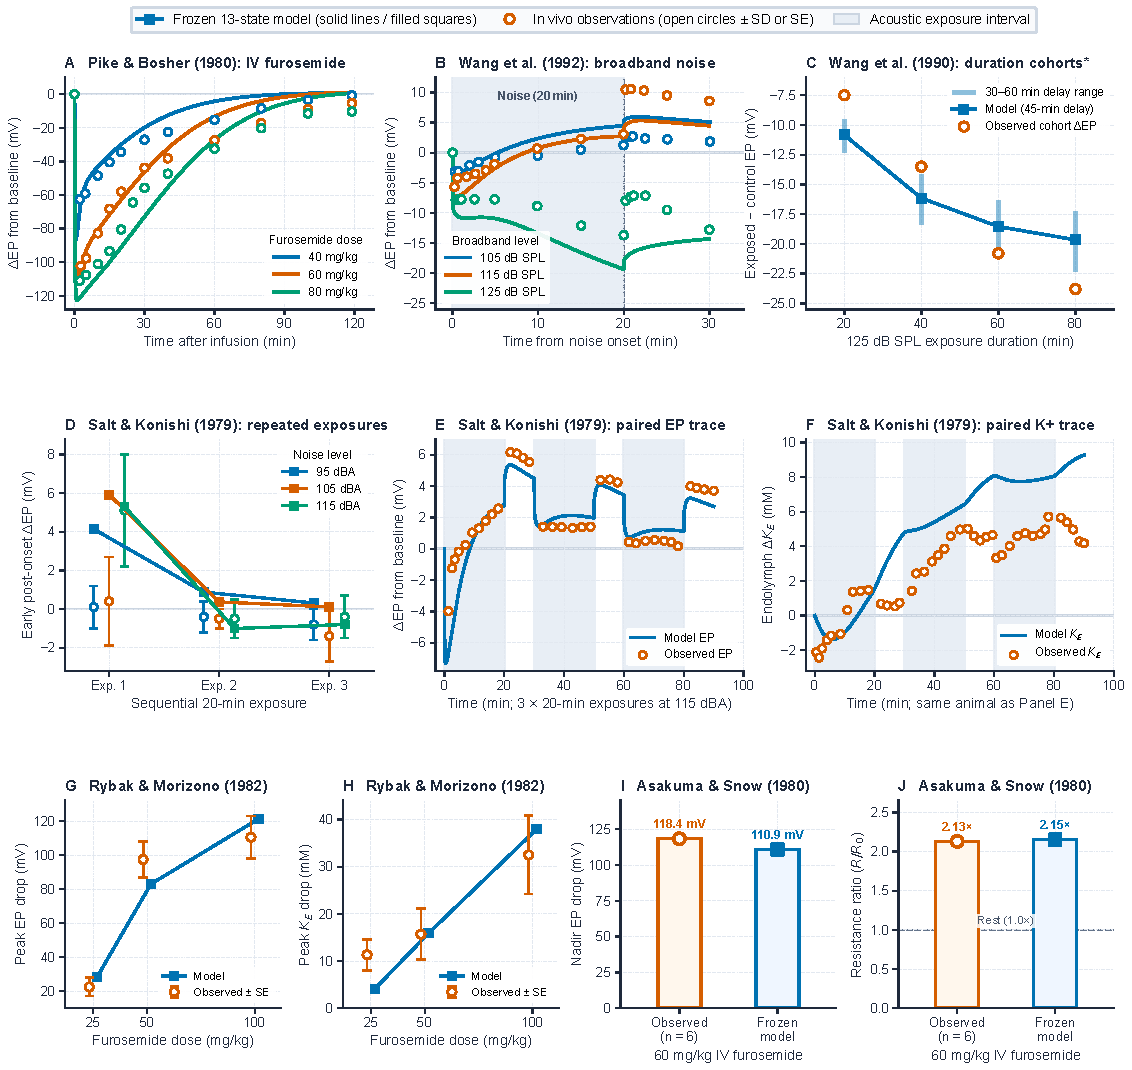
\includegraphics[width=\textwidth]{figures/figure1-tier1-joint-fit.pdf}
  \caption{Outcome-informed joint calibration of the 13-state model across six anchoring \emph{in vivo} studies (178 residual targets; one local parameter solution held fixed afterward). \textbf{(A)} \citet{PikeBosher1980} guinea-pig EP time courses following 40, 60, and 80 mg/kg intravenous furosemide (\(n = 2, 3, 3\)). \textbf{(B)} \citet{Wang1992} guinea-pig EP trajectories during and after 20-min broadband noise at 105, 115, and 125 dB SPL; sample sizes are not stated in the source (gray shading marks exposure). \textbf{(C)} \citet{Wang1990} exposed-minus-control cohort EP differences after 20--80 min of 125 dB SPL noise (\(n=20\) per exposure group; control \(n=26\); \emph{protocol-mismatched component}: source measurements included anoxia, which was omitted here; vertical blue bars span the 30--60 min post-noise delay window around the 45-min reference). \textbf{(D)} \citet{SaltKonishi1979} Table III overall post-exposure \(\Delta\mathrm{EP}_o\) summaries across three sequential 20-min exposures at 95, 105, and 115 dBA (source-reported observation counts \(n=3,3,9\), respectively; these are not identified as animal-level sample sizes). The model uses an assumed 1--3-min post-offset window because the source timing is unspecified. \textbf{(E, F)} \citet{SaltKonishi1979} Figure~3 paired \(\Delta\mathrm{EP}\) and endolymphatic \(\Delta K_E\) recordings from one representative animal (\(n=1\)) across three 20-min exposures at 115 dBA (gray bands). \textbf{(G, H)} \citet{RybakMorizono1982} chinchilla peak EP and endolymphatic \(K_E\) reductions at 25, 50, and 100 mg/kg furosemide (bars denote reported SE, \(n = 3, 5, 7\)). \textbf{(I, J)} \citet{AsakumaSnow1980} guinea-pig EP reduction and cochlear partition resistance ratio (\(R/R_0\)) at 60 mg/kg furosemide (\(n = 6\)). Across all panels, solid curves and filled squares represent the model; open circles denote experimental observations. Residual targets and digitized points do not represent additional animals.}
  \label{fig:tier1}
\end{figure*}

In the in-sample descriptive comparison, the frozen reference realization yields rapid EP collapse to negative nadirs and dose-ordered biphasic recovery over 60--120 min in guinea pigs \citep{PikeBosher1980}; the curve RMSEs are \(6.28\), \(7.02\), and \(10.34\,\mathrm{mV}\) at 40, 60, and 80 mg/kg, respectively (Fig.~\ref{fig:tier1}A). In chinchillas, the simulated peak EP reductions of \(28.5\), \(83.0\), and \(121.3\,\mathrm{mV}\) compare with observed reductions of \(22.3\), \(97.4\), and \(110.5\,\mathrm{mV}\), while the simulated endolymphatic potassium reductions of \(4.09\), \(15.91\), and \(37.94\,\mathrm{mM}\) compare with observed values of \(11.3\), \(15.7\), and \(32.5\,\mathrm{mM}\) \citep{RybakMorizono1982} (Fig.~\ref{fig:tier1}G, H). At 60 mg/kg, the simulated nadir EP drop is \(110.9\,\mathrm{mV}\), compared with \(118.4\,\mathrm{mV}\) observed, and the simulated partition-resistance ratio is \(2.155\), compared with \(2.13\) observed \citep{AsakumaSnow1980} (Fig.~\ref{fig:tier1}I, J). These in-sample numerical correspondences describe this selected objective and do not estimate predictive performance.

For the acoustic targets, the model output shows moderate-level EP stability or rebound at 105 and 115 dB SPL, but its simulated \(19.35\,\mathrm{mV}\) decline at 125 dB SPL exceeds the approximately \(13.7\,\mathrm{mV}\) decline digitized at the 20-min endpoint in \citet{Wang1992}; the delayed post-exposure recovery slope is also underpredicted (Fig.~\ref{fig:tier1}B). The output shows monotonic duration dependence across the four 20--80 min targets from \citet{Wang1990}, although those targets include an unmodeled anoxia challenge (Fig.~\ref{fig:tier1}C). The three-exposure Salt and Konishi Table III summary is compared under the assumed 1--3-min post-offset observation window (Fig.~\ref{fig:tier1}D); the source does not establish that timing. For the paired recordings in Figure~3 of that study, which are from one representative animal (\(n=1\)), the in-sample RMSE is \(1.28\,\mathrm{mV}\) for \(\Delta\mathrm{EP}\) and \(2.81\,\mathrm{mM}\) for endolymphatic potassium accumulation \(\Delta K_E\) across three consecutive 115-dBA exposures (Fig.~\ref{fig:tier1}E, F).

Importantly, presenting all 10 calibration panels side by side in Fig.~\ref{fig:tier1} also makes cross-study tensions immediately transparent. In particular, the model predicts an initial transient EP dip during the first minutes of 105--115 dB SPL noise followed by an intra-exposure climb (driven by rapid adaptation \(\alpha\) reducing MET load \(m\)), which matches the repeated-exposure adaptation in \citet{SaltKonishi1979} Figure~3 (Fig.~\ref{fig:tier1}E) but overpredicts the first-exposure positive \(\Delta\mathrm{EP}\) at 95 dBA in \citet{SaltKonishi1979} Table III (Fig.~\ref{fig:tier1}D) and underpredicts the delayed post-exposure recovery slope in \citet{Wang1992} at 125 dB SPL (Fig.~\ref{fig:tier1}B).

\subsection{Parameter freezing, local residual geometry, and exclusion sensitivity analysis}\label{sec:calibration-freeze}

Following the joint six-study fit, the nine calibrated parameters were frozen at their selected local solution: guinea-pig dose proxy \(d_{\mathrm{GP}} = 0.048828432\,\mathrm{proxy}\cdot(\mathrm{mg/kg})^{-1}\), chinchilla multiplier \(s_{\mathrm{Ch}} = 0.78623755\), furosemide conductance loss \(\ell_D = 0.94916493\), diuretic potassium-loss coefficient \(\ell_D^K = 0.012931172\,V_{E,0}\,\mathrm{min}^{-1}\), slow drug washout fraction \(f_{\mathrm{slow}} = 0.68775697\), slow washout time constant \(\tau_{\mathrm{slow}} = 59.380317\,\mathrm{min}\), adaptation accumulation rate \(r_\alpha^{\mathrm{rate}} = 0.14823975\,\mathrm{min}^{-1}\), evoked adaptation weight \(e_\alpha = 0.94641389\), and trauma-associated vasoconstriction \(\rho_W = 0.20000000\). Eight parameters lie inside their admissible boxes; \(\rho_W\) is at its declared lower bound of \(0.20\). This 80-entry reference vector is held fixed across the reported diagnostics and benchmarks; the word ``frozen'' describes post-fit handling, not evidence that the solution is uniquely identified.

To characterize the local geometry of the calibration objective around the selected solution, we evaluated the \(178 \times 9\) weighted residual Jacobian \(J\) in normalized unit-box coordinates using finite-difference steps of \(10^{-3}\) and \(5 \times 10^{-4}\) (with one-sided differences at the active \(\rho_W\) lower bound). Both step sizes yielded similar singular-value spectra spanning \(\sigma_{\max} = 85.98\) down to \(\sigma_{\min} = 0.2269\), corresponding to a scaled condition number of \(\kappa(J) = 378.9\). The strongest pairwise collinearity occurred between the slow washout fraction \(f_{\mathrm{slow}}\) and slow washout time constant \(\tau_{\mathrm{slow}}\) (column cosine \(= 0.844\)). The weakest singular direction aligned almost entirely with \(\rho_W\), whose directional objective gradient at the lower bound was positive (\(+0.386\) per unit-box coordinate). This local derivative diagnostic is conditional on the selected residual scales and does not provide parameter intervals or global identifiability. Profile-objective curves, bootstrap and multi-study leave-one-out refits, and alternative-weight refits were not completed; no confidence intervals are reported.

Because the four targets from \citet{Wang1990} involved an unmodeled anoxia challenge, we also performed a dedicated five-study exclusion refit (retaining 174 targets across the remaining five studies) starting from the frozen reference. Removing \citet{Wang1990} changed the retained five-study weighted sum of squared residuals from \(19.906813\) at the freeze to \(19.906702\) after refitting (a decrease of \(1.11\times10^{-4}\), smaller than the fine-grid change of \(0.0306\)), left \(\rho_W = 0.200\) unchanged at its lower bound, and shifted \(r_\alpha^{\mathrm{rate}}\) (\(0.14824 \to 0.14694\,\mathrm{min}^{-1}\)) and \(e_\alpha\) (\(0.94641 \to 0.95139\)) by less than \(0.9\%\). Thus, this one protocol-exclusion refit changed the weighted objective very little; it does not establish robustness to other study exclusions or alternative weights.

\section{Stability analysis and flux-budget diagnostics}\label{sec:stability}

A dynamical audit of the frozen candidate examined local Jacobian eigenvalues, selected finite-horizon perturbations, internal state trajectories, and equation-level flux budgets (Figs.~\ref{fig:diagnostics} and~\ref{fig:scenario-states}). The 13-state system contains nonsmooth switching functions (\(\max(0,\cdot)\) in \(a_r\), \(e\), \(I_{\mathrm{circ}}\), \(M\), and \(\Delta g\)) and a potassium-inventory state \(N_K\); these diagnostics do not establish global stability or physiological validity.

\begin{figure*}[!t]
  \centering
  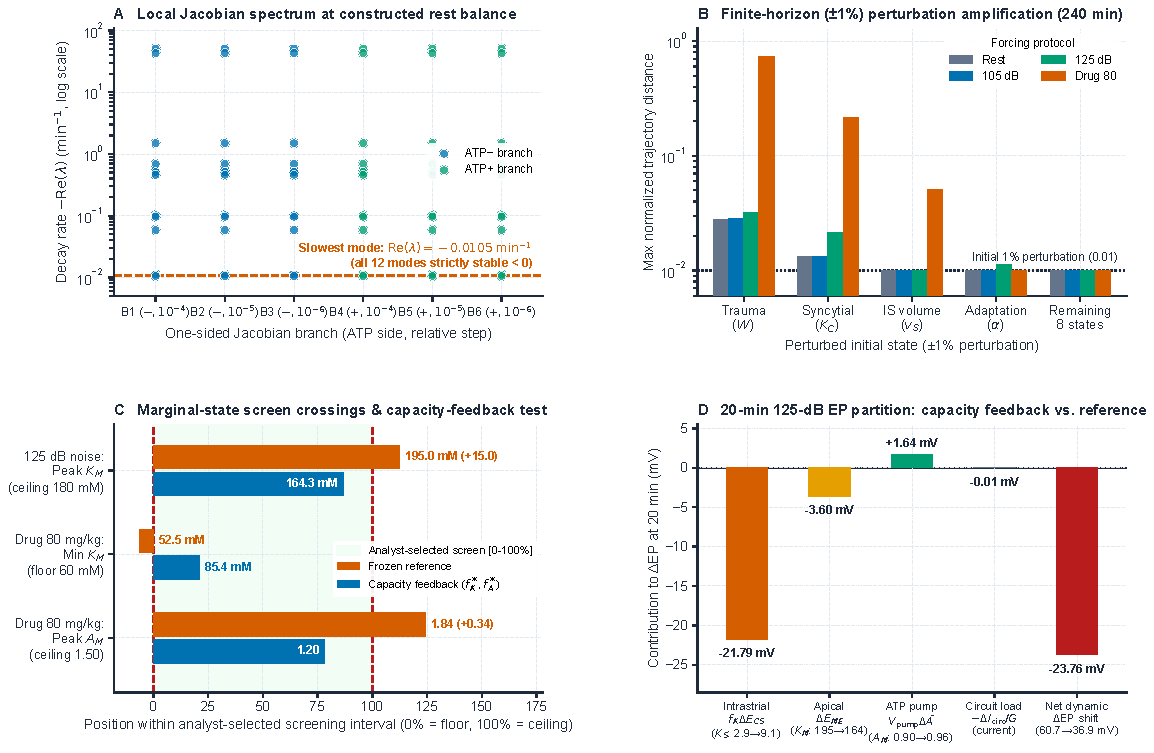
\includegraphics[width=\textwidth]{figures/figure2-stability-and-model-only-forecast.pdf}
  \caption{Local Jacobian eigenvalues, finite-horizon perturbation amplification, and equation-level flux-budget diagnostics of the frozen 13-state model. \textbf{(A)} Decay rates \(-\mathrm{Re}(\lambda_i)\) (log scale, \(\mathrm{min}^{-1}\)) of the 12 non-conserved eigenmodes across six one-sided finite-difference Jacobian approximations evaluated on both sides of the resting endolymphatic ATP branch (\(a < a_0\) in blue; \(a > a_0\) in green) at relative steps of \(10^{-4}\), \(10^{-5}\), and \(10^{-6}\). The 12 modes comprise two fastest, five intermediate, three slower, and two slowest modes; all have negative real parts in these branch-specific approximations. The slowest is \(\mathrm{Re}(\lambda_{\max}) = -0.0105\,\mathrm{min}^{-1}\) (dashed orange line). \textbf{(B)} Maximum scaled trajectory distance from matched controls over a 240-min horizon following single-state \(1\%\) initial perturbations across quiet rest, 105-dB SPL noise, 125-dB SPL noise, and 80-mg/kg furosemide forcing. \textbf{(C)} Position of extreme sampled marginal-cell states (\(K_M\) and \(A_M\)) relative to analyst-selected screening ranges (crimson dashed lines mark the 60-mM floor and 180-mM / 1.50 screening levels; the \(A_M\) value is a normalized proxy, not an empirical physiological ceiling), comparing the frozen reference (orange bars, showing three threshold crossings) against the uncalibrated capacity-feedback counterfactual (\(f_K^*, f_A^*\); blue bars, keeping sampled states within those screens). \textbf{(D)} Quasi-steady circuit voltage partition at \(t = 20\,\mathrm{min}\) during 125-dB SPL noise, showing that the counterfactual deepens the EP nadir by \(-23.76\,\mathrm{mV}\) (\(60.65 \to 36.89\,\mathrm{mV}\)) primarily through intrastrial potassium retention (\(K_S: 2.92 \to 9.12\,\mathrm{mM}\)) and loss of the intermediate-cell diffusion battery (\(f_K\Delta E_{CS} = -21.79\,\mathrm{mV}\)).}
  \label{fig:diagnostics}
\end{figure*}

\subsection{Local Jacobian eigenvalue spectra across nonsmooth switching branches}\label{sec:stability-spectra}

At the constructed quiet rest balance (with conserved potassium inventory \(N_K = 212.1425\,\mathrm{mM}\,V_{E,0}\)), the maximum scaled time derivative across all 13 states was \(4.9 \times 10^{-13}\,\mathrm{min}^{-1}\), confirming a numerical steady state to machine precision. Because the subtectorial ATP amplification law \(a_r = a_0 + c_a\max(0, a - a_0)\) and excess drive \(e = \max(0, q - 1)\) possess one-sided directional derivatives at the resting threshold \(a = a_0\), we evaluated six one-sided \(12 \times 12\) reduced Jacobian matrices (holding conserved \(N_K\) fixed) across both the sub-baseline (\(a - a_0 < 0\)) and super-baseline (\(a - a_0 > 0\)) ATP branches at relative perturbation steps of \(10^{-4}\), \(10^{-5}\), and \(10^{-6}\).

As shown in Fig.~\ref{fig:diagnostics}A, all 12 eigenvalues across the six branch approximations were strictly real and negative, spanning more than three orders of magnitude in relaxation rate. The two fastest modes, \(\lambda_1=-51.33\,\mathrm{min}^{-1}\) (\(\tau\approx1.17\,\mathrm{s}\)) and \(\lambda_2=-43.31\,\mathrm{min}^{-1}\) (\(\tau\approx1.39\,\mathrm{s}\)), correspond to intrastrial potassium turnover and transepithelial circuit-capacitance relaxation, respectively. Five intermediate modes range from \(-1.50\) to \(-0.460\,\mathrm{min}^{-1}\) (\(\tau\approx0.67\)--\(2.17\,\mathrm{min}\)) and reflect ATP clearance, perfusion, and cellular ATP turnover. Three slower modes at \(-0.1015\), \(-0.0962\), and \(-0.0585\,\mathrm{min}^{-1}\) (\(\tau\approx9.9\)--\(17.1\,\mathrm{min}\)) correspond to intrastrial volume restoration and potassium redistribution. The two slowest modes are \(\lambda_{11}=-0.01111\,\mathrm{min}^{-1}\) (\(\tau_\alpha=90.0\,\mathrm{min}\)) and \(\lambda_{12}=-0.01053\,\mathrm{min}^{-1}\) (\(\tau_R=95.0\,\mathrm{min}\)).
The negative real parts across the calculated one-sided branch Jacobians support local linear stability at the constructed resting balance. They do not prove nonlinear stability across switching surfaces, global attraction, or stability under arbitrary forcing.

\subsection{Finite-horizon perturbation amplification across resting and forced protocols}\label{sec:stability-perturbations}

To examine selected nonlinear responses, we integrated Radau and BDF trajectories for 240 min after single-state \(1\%\) perturbations of each of the 12 non-inventory states from the solved resting balance, under quiet rest and three forced protocols: 105-dB and 125-dB broadband noise for 20 min and 80-mg/kg intravenous furosemide (Fig.~\ref{fig:diagnostics}B). For adaptation and trauma, which begin at a lower boundary, only the positive perturbation was used; the other 10 states were perturbed in both directions. This gives 22 perturbation directions per protocol and 88 perturbed initial-condition/protocol combinations; each was integrated with both solvers (176 perturbed trajectories). Four matched-control trajectories per solver add eight integrations, for 184 trajectories total; this count excludes local Jacobian evaluations. The matched-control distance at each output time was the scaled infinity norm
\[
d(t)=\max_i \frac{|x_i(t)-x_i^{\mathrm{control}}(t)|}{s_i},
\]
where \(s_i\) is the corresponding state magnitude at the solved resting balance, except that adaptation and trauma use \(s_i=1\); the potassium-inventory state is included in the maximum. Outputs were sampled every \(0.25\,\mathrm{min}\) (961 points), with solver tolerances \(10^{-8}\) and \(10^{-10}\). The largest final distances at 240 min across the single-state perturbations were \(1.47\times10^{-3}\) for 105-dB noise, \(7.52\times10^{-4}\) for 125-dB noise, and \(2.43\times10^{-3}\) for the furosemide protocol; the largest transient distances were \(0.0284\), \(0.0318\), and \(0.737\), respectively. Thus the trajectories did not all return to numerical identity with their controls by 240 min. These finite-horizon results describe tested perturbations only; the residual separation is compatible with slow relaxation and does not establish asymptotic convergence or global boundedness.

Tracking the peak transient divergence \(\max_{t \in [0,240]} \|\Delta \mathbf{x}(t)\|_{\mathrm{norm}}\) across states revealed protocol-dependent amplification (Fig.~\ref{fig:diagnostics}B). For eight states (\(F, O, A_C, A_M, K_S, K_M, V,\) and \(a\)), initial \(1\%\) perturbations decayed monotonically across all four protocols, with a peak distance of \(0.0100\). Under quiet rest and 105 dB SPL noise, perturbations to \(W\) and \(K_C\) showed mild transient amplification, reaching \(0.0281\)--\(0.0284\) and \(0.0133\), respectively. At 125 dB SPL, the corresponding peaks were \(0.0318\) for \(W\), \(0.0215\) for \(K_C\), and \(0.0112\) for \(\alpha\). The strongest transient amplification occurred during the 80 mg/kg furosemide protocol, when \(J_U\) and \(g_S\) are suppressed by approximately \(95\%\): perturbations to \(W\), \(K_C\), and \(v_S\) reached normalized distances of \(0.737\), \(0.215\), and \(0.0508\), respectively, before decaying during drug recovery. This response reflects nonlinear coupling between syncytial--intrastrial potassium gradients and intrastrial edema when marginal clearance is transiently reduced.

\subsection{Dense multi-state trajectories under generic broadband sound scenarios}\label{sec:stability-scenarios}

To inspect the internal state dynamics of the frozen model across sound intensities, we simulated 20-min broadband noise exposures at 105, 115, and 125 dB SPL followed by 100 min of quiet recovery, sampling all states at dense 0.25-min intervals (Fig.~\ref{fig:scenario-states}).

\begin{figure*}[!t]
  \centering
  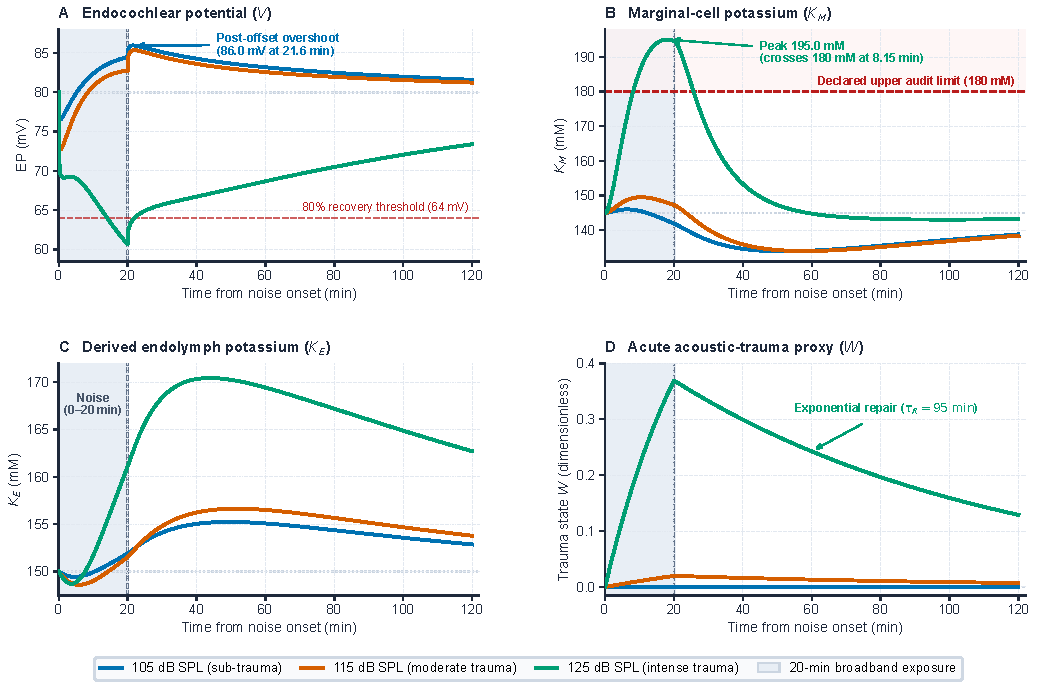
\includegraphics[width=0.92\textwidth]{figures/figure3-model-only-scenario-states.pdf}
  \caption{Dense internal state trajectories of the frozen 13-state model during 20-min broadband noise exposure (gray shaded region, 0--20 min) and 100-min quiet recovery (20--120 min) at 105 dB SPL (blue), 115 dB SPL (orange), and 125 dB SPL (green), sampled at 0.25-min intervals. \textbf{(A)} Endocochlear potential \(V(t)\), illustrating initial sound-onset dips, intra-exposure adaptation recovery, post-offset overshoots at 105 and 115 dB SPL (\(+5.96\) and \(+5.36\,\mathrm{mV}\) above the 80 mV baseline), and deep trauma-driven depression at 125 dB SPL (crossing the 80\% recovery threshold of 64 mV at \(21.94\,\mathrm{min}\)). \textbf{(B)} Marginal-cell intracellular potassium concentration \(K_M(t)\), highlighting its crossing of the analyst-selected 180-mM upper screening level (crimson dashed line and pink shaded zone; peak \(195.04\,\mathrm{mM}\)) during 125 dB SPL exposure. These screening levels are diagnostics, not enforced state bounds. \textbf{(C)} Algebraically derived endolymphatic potassium concentration \(K_E(t)\). \textbf{(D)} Reversible acute acoustic-trauma proxy \(W(t)\), demonstrating the steep threshold recruitment between 115 and 125 dB SPL and slow post-exposure exponential decay (\(\tau_R = 95\,\mathrm{min}\)).}
  \label{fig:scenario-states}
\end{figure*}

At 105 and 115 dB SPL, sound onset produces an immediate circuit-loading dip in EP (minimum drops of \(-3.23\) and \(-7.01\,\mathrm{mV}\)), followed by intra-exposure recovery as purinergic P2X2 activation and transducer adaptation \(\alpha\) attenuate the effective MET conductance factor \(m(t)\). At sound offset (\(t = 20\,\mathrm{min}\)), when the evoked acoustic drive \(e(t)\) vanishes instantaneously while slow adaptation \(\alpha(t)\) (\(\tau_\alpha = 90\,\mathrm{min}\)) remains elevated, the reduced resting MET load produces a characteristic post-offset EP overshoot to \(85.96\,\mathrm{mV}\) (at \(21.6\,\mathrm{min}\) for 105 dB) and \(85.36\,\mathrm{mV}\) (at \(22.0\,\mathrm{min}\) for 115 dB) before relaxing toward the 80 mV baseline (Fig.~\ref{fig:scenario-states}A; summarized at 20, 40, 60, and 120 min as \(84.48, 84.26, 83.17, 81.58\,\mathrm{mV}\) for 105 dB and \(82.75, 83.60, 82.56, 81.23\,\mathrm{mV}\) for 115 dB).

In contrast, at 125 dB SPL, excess drive exceeds the steep trauma threshold (\(K_W = 0.272, n_W = 14\)), driving \(W(t)\) to \(0.369\) at 20 min (Fig.~\ref{fig:scenario-states}D). Trauma recruitment triggers internal paracellular potassium leakage (\(\ell_W W\)) from the syncytium into the intrastrial space, depressing EP to a nadir of \(60.65\,\mathrm{mV}\) (\(-19.35\,\mathrm{mV}\) drop; returning above the 64 mV 80\%-of-baseline threshold at \(21.94\,\mathrm{min}\) and reaching \(66.72, 68.69, 73.39\,\mathrm{mV}\) at 40, 60, and 120 min; Fig.~\ref{fig:scenario-states}A). Concurrently, elevated intrastrial potassium stimulates rapid basolateral marginal uptake \(J_U\), driving marginal-cell potassium \(K_M(t)\) up to a peak of \(195.04\,\mathrm{mM}\) during exposure (Fig.~\ref{fig:scenario-states}B) and subsequently elevating endolymphatic potassium \(K_E(t)\) to \(170.45\,\mathrm{mM}\) during early recovery (Fig.~\ref{fig:scenario-states}C).

\subsection{Equation-level flux-budget diagnostics of marginal-state range excursions}\label{sec:stability-flux-budgets}

Comparing the sampled trajectories with the declared screening ranges revealed three threshold crossings under severe forcing: one during 125 dB SPL noise (\(K_M > 180\,\mathrm{mM}\)) and two during 80 mg/kg furosemide (\(K_M < 60\,\mathrm{mM}\) and \(A_M > 1.50\); Fig.~\ref{fig:diagnostics}C). These are analyst-selected diagnostic screens, not enforced constraints or empirically established physiological bounds. In particular, \(A_M\) is a dimensionless ATP-availability proxy normalized to one at rest; the 1.50 ceiling is a chosen screening level, not a measured ATP concentration or demonstrated physiological maximum. The crossings therefore flag unbounded-by-design effective states, not proof that the biological concentrations are impossible. The Wang et al. (1992) 125-dB and Pike and Bosher 80-mg/kg protocols also contribute to the calibration objective, which does not penalize internal screening-range crossings. Thus, some endpoint fits rely on trajectories whose internal-state plausibility is unresolved; no constrained or range-penalized refit has been performed. We evaluated the differential flux budgets \(\phi_M \dot{K}_M = J_U - J_A\) and \(\tau_M \dot{A}_M = S_M - C_M\), where \(S_M = 2O_x/[1 + A_M/A_0]\), at 0.05-min resolution. During 125 dB SPL noise, trauma-induced paracellular leak \(\ell_W W(K_C - K_S)\) elevates \(K_S\), activating the Michaelis--Menten uptake term \(U_M(K_S)\) in Eq.~(\ref{eq:um}). At \(t=8.15\,\mathrm{min}\), \(K_M\) crosses the 180-mM screen and rises to \(195.04\,\mathrm{mM}\). Basolateral uptake is \(J_U=3.630\,\mathrm{mM}\,V_{E,0}\,\mathrm{min}^{-1}\), compared with linear apical secretion \(J_A=q_K(K_M/K_{M,0})=3.478\,\mathrm{mM}\,V_{E,0}\,\mathrm{min}^{-1}\). With the marginal-cell volume ratio \(\phi_M=0.042\) held constant and no osmotic swelling or KCNQ1 saturation feedback, this net flux imbalance of \(+0.152\,\mathrm{mM}\,V_{E,0}\,\mathrm{min}^{-1}\) produces a concentration increase of \(\dot{K}_M=+3.609\,\mathrm{mM}\,\mathrm{min}^{-1}\).

During 80 mg/kg furosemide exposure, the decrease in \(h_D\) reduces marginal-cell uptake \(J_U=q_Kh_DU_M\) to \(0.800\,\mathrm{mM}\,V_{E,0}\,\mathrm{min}^{-1}\) at \(t=3.10\,\mathrm{min}\). Apical secretion remains \(1.157\,\mathrm{mM}\,V_{E,0}\,\mathrm{min}^{-1}\), continuing to deplete \(K_M\) in proportion to \(K_M/K_{M,0}\). Consequently, \(K_M\) crosses the \(60\,\mathrm{mM}\) floor at \(t=3.10\,\mathrm{min}\), reaches \(52.46\,\mathrm{mM}\), and initially declines at \(\dot{K}_M=-8.489\,\mathrm{mM}\,\mathrm{min}^{-1}\) before equilibrating with the reduced uptake.

The same furosemide exposure causes \(A_M\) to cross the 1.50 screening level at \(t=1.65\,\mathrm{min}\), reaching 1.839. Because Eq.~(\ref{eq:cm}) assigns active transport a weight of \(\eta_M=0.78\), inhibition of \(h_DU_M\) removes a major ATP sink. At the crossing, oxidative synthesis \(S_M=0.801\) exceeds the combined housekeeping (\(0.330\)) and transport (\(0.155\)) consumption terms, yielding \(\dot{A}_M=+0.211\,\mathrm{min}^{-1}\). This reflects ATP sparing when \(\mathrm{Na}^+/\mathrm{K}^+\)-ATPase/NKCC1 cycling is inhibited and also indicates that the simplified synthesis law \(2O_x/(1 + A_M/A_0)\) lacks tight allosteric product inhibition.

\subsection{Counterfactual tests of marginal capacity feedback and potassium boundary conservation}\label{sec:stability-counterfactuals}

To test whether simple local feedback modifications can eliminate these range excursions without altering the rest of the model, we evaluated an uncalibrated \emph{capacity-feedback counterfactual} in which marginal potassium uptake \(J_U\) and marginal ATP synthesis \(S_M\) are multiplied by soft saturation factors approaching zero at the declared audit ceilings (\(180\,\mathrm{mM}\) and \(1.50\) relative ATP units):
\begin{equation}
  f_K^* = \frac{\max(0, 180 - K_M)}{180 - K_{M,0}}, \qquad
  f_A^* = \frac{\max(0, 1.5 - A_M)}{1.5 - A_0},
  \label{eq:capacity-feedback}
\end{equation}
applied consistently across \(J_U\) in Eqs.~(\ref{eq:dks}), (\ref{eq:dkm}), and (\ref{eq:cm}) without clipping state variables or refitting parameters.

As shown in Fig.~\ref{fig:diagnostics}C (blue bars), introducing \(f_K^*\) and \(f_A^*\) eliminated the declared-range violations across both protocols (Radau--BDF solver agreement \(<6.7\times10^{-7}\)). Peak noise-driven \(K_M\) was bounded at \(164.25\,\mathrm{mM}\), minimum drug-driven \(K_M\) increased to \(85.37\,\mathrm{mM}\), and peak drug-driven \(A_M\) was \(1.195\). However, restricting marginal potassium uptake during 125 dB SPL noise deepened the 20-min EP nadir by \(23.76\,\mathrm{mV}\), from \(60.65\,\mathrm{mV}\) in the frozen reference to \(36.89\,\mathrm{mV}\) in the counterfactual.

To quantify the mechanism underlying this \(-23.76\,\mathrm{mV}\) shift, we partitioned the instantaneous circuit-equilibrium voltage \(V_{\mathrm{eq}} = (g_S V_S + g_{\mathrm{MET}}m V_{\mathrm{MET}} + g_P V_P)/(g_S + g_{\mathrm{MET}}m + g_P)\) at \(t = 20\,\mathrm{min}\) between the frozen reference and capacity-feedback trajectories (Fig.~\ref{fig:diagnostics}D). Throttling marginal uptake via \(f_K^*\) reduces \(J_U\) from \(3.745\) to \(3.172\,\mathrm{mM}\,V_{E,0}\,\mathrm{min}^{-1}\), causing unextracted potassium to back up inside the narrow intrastrial space from \(K_S = 2.923\,\mathrm{mM}\) (reference) to \(9.123\,\mathrm{mM}\) (counterfactual). This three-fold rise in \(K_S\) collapses the intermediate-cell Kir4.1 diffusion battery from \(E_{CS} = 96.60\,\mathrm{mV}\) to \(67.35\,\mathrm{mV}\), contributing \(-21.790\,\mathrm{mV}\) to \(\Delta\mathrm{EP}\), alongside \(-3.605\,\mathrm{mV}\) from the apical battery \(\Delta E_{ME}\), \(+1.642\,\mathrm{mV}\) from direct ATP voltage, and \(-0.012\,\mathrm{mV}\) from circuit load (total quasi-steady sum: \(-23.765\,\mathrm{mV}\) vs.\ actual dynamic \(\Delta\mathrm{EP} = -23.762\,\mathrm{mV}\); Fig.~\ref{fig:diagnostics}D). In this uncalibrated counterfactual, limiting marginal-cell uptake without changing the model's fixed-volume and apical-secretion terms produces an intrastrial potassium rise and a large EP shift. This is a consequence of the selected compartments, flux laws, and feedback factors; it does not establish a general physiological principle or an experimentally demonstrated mechanism.

Finally, two \emph{boundary-exchange counterfactuals} were tested using Eq.~(\ref{eq:jperi}) with all parameters frozen. Sealing the perilymphatic potassium boundary during 80 mg/kg furosemide (\(\mathbf{1}_{\mathrm{drug}}=0\)) conserved \(N_K=212.1425\) rather than permitting a loss of \(8.049\,\mathrm{mM}\,V_{E,0}\) units; this changed the 240-min EP trajectory by at most \(6.97\,\mathrm{mV}\) and prevented endolymphatic \(K_E\) depletion. Enabling the same exchange law continuously during 125 dB SPL noise produced a net inventory loss of \(10.031\,\mathrm{mM}\,V_{E,0}\) units and a maximum EP shift of \(2.02\,\mathrm{mV}\), while leaving the marginal \(K_M\) and \(A_M\) excursions intact. In this model, protocol-conditioned potassium gating alters macroscopic endolymphatic potassium balance, while the marginal-cell range excursions reflect its selected uptake--secretion coupling.

\section{Retrospective comparisons and vascular scenario analysis using Zhang and Hou studies}\label{sec:benchmarks}

\subsection{Rationale and transfer protocol for unfitted retrospective benchmarks}\label{sec:benchmarks-rationale}

With the 80 model entries held fixed after the six-study calibration, we compared model outputs with observations from \citet{Zhang2021} and \citet{Hou2020}, neither of which contributed residuals to the fit. Both studies were available during model development, and transfer mappings or interpretations were selected after inspection; these are retrospective, outcome-informed comparisons, not independent or blinded validation. \citet{Zhang2021} recorded ISP, intrastrial potassium (\([\mathrm{K}^+]_{\mathrm{IS}}\)), and EP responses to 10-s 1-kHz pure-tone bursts (60--100 dB SPL) in the second cochlear turn of guinea pigs. \citet{Hou2020} quantified strial capillary blood flow and EP after intense broadband noise exposure (120 dB SPL, 3 h/day for 2 consecutive days) and pericyte transplantation in mice.

\subsection{Dynamic tone-level potassium mismatch and conditional voltage agreement (Zhang et al., 2021)}\label{sec:benchmarks-zhang}

To simulate the descending tone-level protocol of \citet{Zhang2021} Figure~5 (four 10-s 1-kHz tone pulses with 0.5-s linear ramps separated by 30-s quiet intervals at 100, 90, 80, 70, and 60 dB SPL, carried forward continuously without state resets), we compared two acoustic input mappings. The \emph{direct broadband transfer} applies the frozen broadband SPL transform \(q(L)\) in Eq.~(\ref{eq:sound-map}) to the nominal tone levels. The alternative \emph{outcome-informed tone-drive mapping} uses \(q=1.131, 1.095, 1.071, 1.047,\) and \(1.028\) for 100--60 dB SPL in Figure~5 and \(q=1.076\) for the separate 90-dB cohort in Figure~4. These tone-drive values were selected after examining the reported voltage responses and therefore cannot be treated as an independent transfer prediction.

\begin{figure*}[!t]
  \centering
  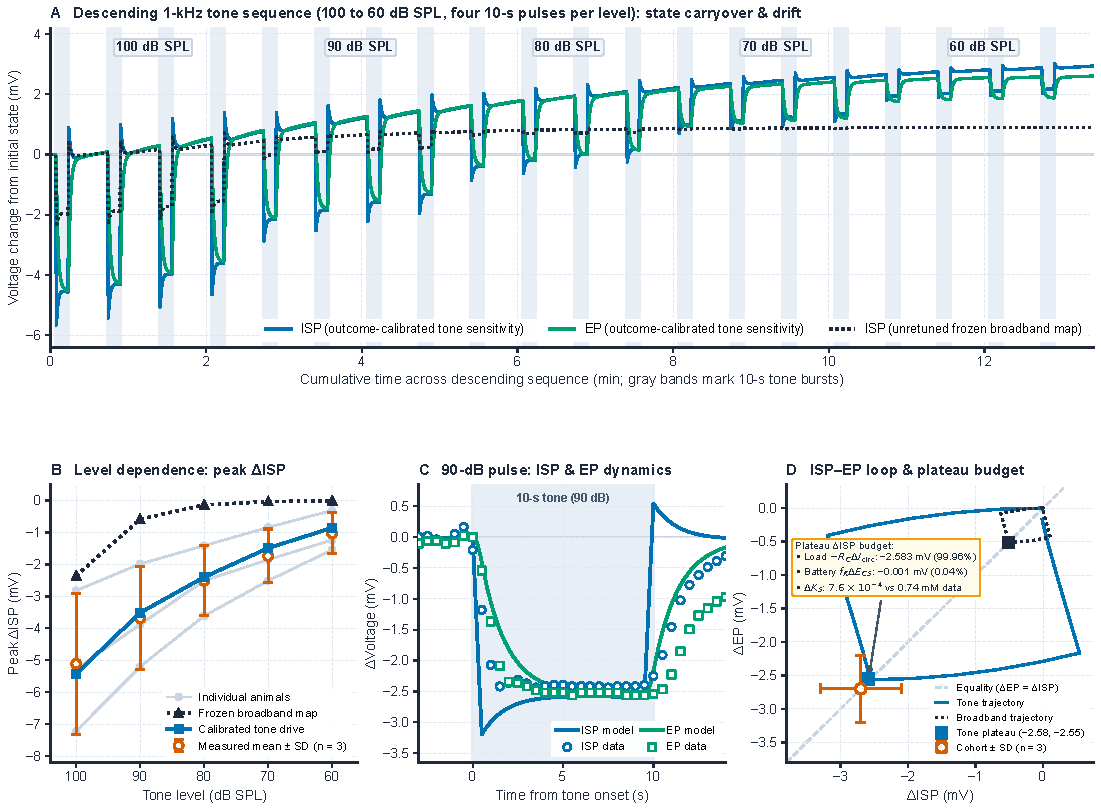
\includegraphics[width=\textwidth]{figures/figure4-zhang-retrospective-benchmark.pdf}
  \caption{Retrospective, outcome-informed comparison of the frozen 13-state model with 1-kHz tone-burst recordings in the guinea-pig cochlear lateral wall from \citet{Zhang2021}. The primary discrepancy is an approximately three-order-of-magnitude underprediction of the representative potassium transient; voltage agreement is conditional on the outcome-informed tone-drive mapping. \textbf{(A)} Simulated continuous descending level sequence (100, 90, 80, 70, and 60 dB SPL; four 10-s tone bursts per level marked by gray vertical bands, with 30-s quiet intervals and full state carryover), comparing ISP (blue) and EP (green) under the outcome-informed tone-drive mapping against ISP under the unretuned broadband map (dotted dark line). \textbf{(B)} Peak four-pulse averaged \(\Delta\mathrm{ISP}\) across descending sound levels, comparing digitized three-animal means \(\pm\) SD (open orange circles; thin gray lines show individual animals from \citealt{Zhang2021}, Fig.~5E) with the frozen broadband map (dotted black triangles) and outcome-informed tone drive (solid blue squares). \textbf{(C)} Digitized 10-s 90-dB SPL ISP and EP traces from a representative animal (GP267; four-pulse average) in \citet{Zhang2021} Figure~4E, with model trajectories. \textbf{(D)} Parametric \(\Delta\mathrm{ISP}\)--\(\Delta\mathrm{EP}\) phase-plane loop during the 90-dB pulse (filled squares mark 7--9 s plateau averages) plotted against the published cohort means \(\pm\) SD (\(-2.7 \pm 0.6\,\mathrm{mV}\) ISP, \(-2.7 \pm 0.5\,\mathrm{mV}\) EP, \(n = 3\); open orange circle). The representative intrastrial potassium trace in the source is from a sequential electrode-position recording, not simultaneous with these voltage recordings. The callout shows that \(99.96\%\) of the modeled \(-2.584\,\mathrm{mV}\) plateau ISP deflection arises from resistive circuit loading (\(-R_C\Delta I_{\mathrm{circ}}\)) rather than intrastrial diffusion-battery modulation (\(f_K\Delta E_{CS}\)); this conditional voltage decomposition does not explain the measured potassium response.}
  \label{fig:zhang}
\end{figure*}

The principal diagnostic failure is the potassium response. For the 90-dB, 1-kHz tone comparison in Figure~4 of \citet{Zhang2021}, the paper reports a representative intrastrial potassium increase of approximately \(0.74\,\mathrm{mM}\), with a reported response time constant of \(0.8\,\mathrm{s}\); the model's maximum \(\Delta K_S\) is \(7.59\times10^{-4}\,\mathrm{mM}\), roughly three orders of magnitude smaller. The reported measurement and the state \(K_S\) share concentration units and refer to the intrastrial compartment, but the model is spatially lumped and the plotted potassium trace is from one representative animal. The voltage group means (\(n=3\)) and potassium recording were acquired in sequential electrode-position recordings, not simultaneously in the same four-channel measurement. Thus, the comparison establishes a scale discrepancy under the selected tone protocol, not a paired voltage--potassium prediction error for an individual cochlea.

Only after that ionic mismatch is made explicit do the voltage comparisons provide a conditional secondary result. As shown in Fig.~\ref{fig:zhang}A and~\ref{fig:zhang}B, direct application of the frozen broadband map \(q(L)\) (which has an inflection midpoint at \(110.5\,\mathrm{dB}\) SPL) underestimates the sound-evoked ISP drops across 100--60 dB SPL, yielding peak four-pulse averaged changes of \(-2.35, -0.58, -0.13, -0.031,\) and \(-0.0069\,\mathrm{mV}\) versus the digitized three-animal empirical means of \(-5.11 \pm 2.21, -3.69 \pm 1.62, -2.51 \pm 1.10, -1.73 \pm 0.84,\) and \(-1.03 \pm 0.64\,\mathrm{mV}\). With the outcome-informed tone drives, the computed output curve lies near the empirical level dependence (\(-5.42, -3.51, -2.40, -1.49,\) and \(-0.85\,\mathrm{mV}\); Fig.~\ref{fig:zhang}B), and the separate 90-dB simulation yields plateau values near the reported group means: ISP is \(-2.58\,\mathrm{mV}\) versus \(-2.7 \pm 0.6\,\mathrm{mV}\) observed (absolute difference \(0.12\,\mathrm{mV}\), \(4.4\%\) of the observed magnitude), and EP is \(-2.55\,\mathrm{mV}\) versus \(-2.7 \pm 0.5\,\mathrm{mV}\) observed (difference \(0.15\,\mathrm{mV}\), \(5.6\%\); \(n=3\); Fig.~\ref{fig:zhang}C, D). The latter agreement is conditional on the outcome-informed mapping and is not an independent test.

Inspection of the full state trajectories provides additional mechanistic information beyond the plateau voltages. Because \(V_{\mathrm{ISP}}\) in Eq.~(\ref{eq:isp}) responds instantaneously to \(-R_C I_{\mathrm{circ}}\), whereas \(V(t)\) in Eq.~(\ref{eq:voltage}) is filtered by circuit capacitance \(C_V\), simulated ISP falls more rapidly at tone onset, reaching \(-3.20\,\mathrm{mV}\) before relaxing to its \(-2.58\,\mathrm{mV}\) plateau. ISP also shows a positive rebound at tone offset, producing a counterclockwise hysteresis loop in the \(\Delta\mathrm{ISP}\)--\(\Delta\mathrm{EP}\) plane and cumulative upward baseline drift across the 20-pulse sequence as adaptation \(\alpha\) accumulates (Fig.~\ref{fig:zhang}A, C, D).

The voltage--potassium tension can be illustrated, but not resolved, using the model's own Nernst expression \(E_{CS}=V_T\ln(K_C/K_S)\). If \(K_C\) is held fixed and \(K_S\) is changed from the model baseline \(1.5\,\mathrm{mM}\) to the representative observed value \(2.24\,\mathrm{mM}\), the implied change is \(\Delta E_{CS}=V_T\ln(1.5/2.24)\approx-10.7\,\mathrm{mV}\). This is a conditional calculation, not a measured voltage component: the potassium rise and voltage means were not simultaneous paired observations, and it cannot be combined as an empirical decomposition with the model's voltage budget. That budget uses the model-predicted \(\Delta K_S=7.59\times10^{-4}\,\mathrm{mM}\), not the experimental \(0.74\,\mathrm{mM}\) trace, and is conditional on the model's lumped compartments and flux closures.

The voltage budget and flux turnover explain this discrepancy. Decomposition of the algebraic ISP increment
  \begin{equation}
    \Delta V_{\mathrm{ISP}} = f_K \Delta E_{CS} - R_C \Delta I_{\mathrm{circ}}
    \label{eq:isp-budget}
  \end{equation}
over the 7--9 s plateau shows that \(99.96\%\) of the total ISP drop (\(-2.58404\,\mathrm{mV}\)) arises from resistive circulation-current loading (\(-2.58303\,\mathrm{mV}\)); only \(-0.00101\,\mathrm{mV}\) (\(0.04\%\)) is attributable to the intrastrial potassium diffusion battery \(f_K\Delta E_{CS}\) (Fig.~\ref{fig:zhang}D). This small potassium response does not reflect slow turnover. At rest, the intrastrial pool contains \(v_{S,0}K_{S,0}=0.035\times1.5=0.0525\,\mathrm{mM}\,V_{E,0}\), and gross Kir4.1 influx is \(q_K=2.80\,\mathrm{mM}\,V_{E,0}\,\mathrm{min}^{-1}\), corresponding to a gross turnover time of \(1.125\,\mathrm{s}\) (local fixed-other-state relaxation time, \(1.17\,\mathrm{s}\)). Rather, the concentration-gradient surrogate \(J_{\mathrm{Kir}}\) in Eq.~(\ref{eq:jkir}) lacks direct transmembrane voltage driving (\(V_m-E_K\)), while \(J_{\mathrm{para}}=0\) below the trauma threshold. The sound-evoked current must therefore pass through the large syncytial buffer (\(\phi_C=0.40\)) before changing \(J_{\mathrm{Kir}}\). In addition, the small increment in \(K_S\) is rapidly matched by marginal uptake \(J_U\): during the 7--9 s plateau, \(J_{\mathrm{Kir}}\) and \(J_U\) are each approximately \(2.80\,\mathrm{mM}\,V_{E,0}\,\mathrm{min}^{-1}\), with a difference of only \(1.59\)--\(2.02\times10^{-4}\,\mathrm{mM}\,V_{E,0}\,\mathrm{min}^{-1}\) (net-to-gross ratio \(<7.24\times10^{-5}\)).

This retrospective comparison shows that voltage-plateau agreement does not establish that the model represents the underlying potassium-transport mechanism. Under the outcome-informed tone-drive mapping, the lumped circuit produces EP and ISP plateau amplitudes near the reported group means mainly through resistive current loading, but fails to reproduce the magnitude and reported rapid time course of the local intrastrial potassium response. This is a structural limitation of the current compartmental and flux formulation, not a minor secondary error.

\subsection{Retrospective comparison with microvascular injury observations and acute model scenarios (Hou et al., 2020)}\label{sec:benchmarks-hou}

The chronic microvascular observations of \citet{Hou2020} are shown separately from the acute model-generated scenario analysis. In that study, young adult mice exposed to 120 dB SPL broadband noise for 3 h/day on two consecutive days exhibited severe strial capillary degeneration and pericyte-to-myofibroblast transition measured 2--5 weeks post-trauma: untreated noise-exposed mice retained only \(35.5\%\) of control capillary volumetric flow and \(72.0\%\) of control EP (\(72.7 \pm 6.1\,\mathrm{mV}\) vs.\ \(101.0 \pm 4.7\,\mathrm{mV}\), \(n = 3\)), whereas transplantation of control or conditioned pericytes restored flow to \(71.0\%\) and \(90.3\%\) and preserved EP at \(85.1\%\) (\(86.0\,\mathrm{mV}\)) and \(96.8\%\) (\(97.8 \pm 5.5\,\mathrm{mV}\)), respectively (Fig.~\ref{fig:hou}A).

\begin{figure*}[!t]
  \centering
  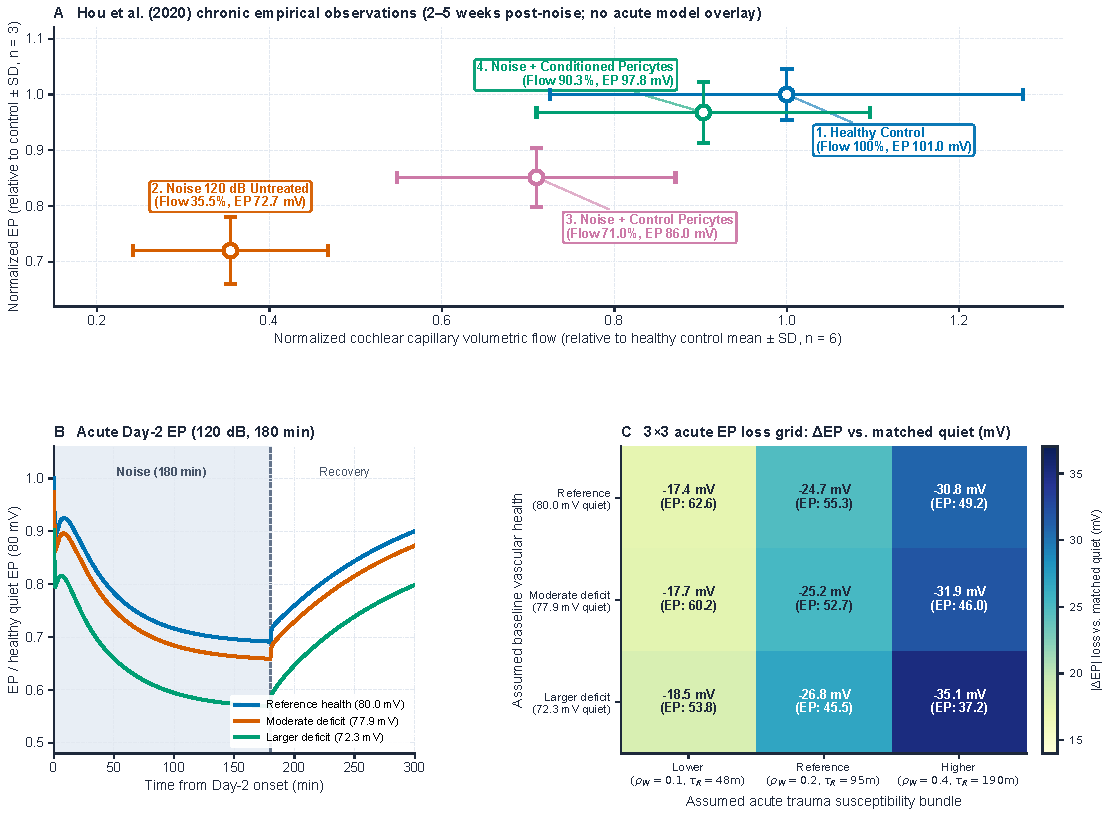
\includegraphics[width=\textwidth]{figures/figure5-hou-vascular-trauma-exploration.pdf}
  \caption{Separation of chronic empirical microvascular-injury observations from \citet{Hou2020} and acute 13-state model susceptibility explorations. \textbf{(A)} Chronic empirical group means \(\pm\) marginal SD for normalized EP (\(n = 3\)) versus normalized strial capillary volumetric blood flow (\(n = 6\)) across all four experimental groups in \citet{Hou2020} Figure~7 (1: healthy control; 2: 120 dB SPL noise untreated; 3: noise plus control pericytes; 4: noise plus conditioned pericytes; recorded 2--5 weeks post-exposure). No acute model points are overlaid on these chronic observations. \textbf{(B)} Acute model-predicted EP trajectories (normalized to the 80.0 mV healthy quiet baseline) during and after the second 180-min 120 dB SPL exposure (Day 2, \(t = 1440\text{--}1740\,\mathrm{min}\)) across three assumed baseline vascular-health bundles at reference trauma susceptibility. \textbf{(C)} Complete \(3 \times 3\) factorial sensitivity grid crossing baseline vascular-health bundles (rows) with acute trauma-susceptibility bundles (columns), displaying the noise-minus-matched-quiet EP loss (\(\Delta\mathrm{EP}\) in mV) and absolute end-exposure EP (in parentheses) at the end of the second 180-min exposure (\(t = 1620\,\mathrm{min}\)).}
  \label{fig:hou}
\end{figure*}

Because the acute 13-state model contains no states for weeks-long pericyte loss, capillary rarefaction, or cell-therapy engraftment, its simulations cannot be interpreted as predictions of the chronic 5-week outcomes. The modeled trauma state instead decays exponentially over hours, \(W(t)=W(t_0)\exp[-(t-t_0)/\tau_R]\). Accordingly, chronic observations are presented separately (Fig.~\ref{fig:hou}A) from an acute \(3\times3\) factorial stress test (Fig.~\ref{fig:hou}B, C). This analysis evaluates how baseline deficits in microvascular delivery and autoregulation affect quiet EP and susceptibility to repeated noise trauma.

We crossed three analyst-selected baseline vascular scenarios, varying reference perfusion, oxygen delivery, and autoregulatory gain \((F_0,p_O,\rho)\), with three analyst-selected acute trauma-susceptibility scenarios, varying trauma-associated vasoconstriction and repair time \((\rho_W,\tau_R)\); all other parameters remained fixed. These settings are illustrative perturbations, not measured vascular phenotypes or fitted parameters. The vascular settings were Reference \((1.0,1.0,0.55)\), Moderate deficit \((0.75,0.75,0.35)\), and Larger deficit \((0.50,0.50,0.15)\). The susceptibility settings were Lower \((0.10,47.5\,\mathrm{min})\), Reference \((0.20,95.0\,\mathrm{min})\), and Higher \((0.40,190.0\,\mathrm{min})\). Each model copy was settled in quiet for \(1440\,\mathrm{min}\) and then exposed to the two-day noise schedule of \citet{Hou2020}: 120 dB SPL for \(0\)--\(180\,\mathrm{min}\) on Day 1 and \(1440\)--\(1620\,\mathrm{min}\) on Day 2, followed by observation through \(1740\,\mathrm{min}\). The grid is a model-generated scenario analysis and does not establish that vascular deficits amplify noise injury in vivo.

In this model-generated factorial grid, quiet EP was relatively insensitive to the selected vascular parameter changes, whereas the simulated acute responses differed more (Fig.~\ref{fig:hou}B, C). Under quiet conditions, reducing baseline vascular delivery by \(25\%\) and \(50\%\) lowered settled normalized perfusion to \(0.774\) and \(0.523\), respectively, but reduced resting EP by only \(2.08\,\mathrm{mV}\) (\(77.92\,\mathrm{mV}\)) and \(7.75\,\mathrm{mV}\) (\(72.25\,\mathrm{mV}\)) relative to the \(80.00\,\mathrm{mV}\) reference. Fractional oxygen extraction \(X_F\) (Eq.~\ref{eq:xf}) and metabolic-demand modulation partially buffer cellular ATP at rest in the model.

At reference trauma susceptibility, two 180-min exposures to 120 dB SPL reduced simulated end-exposure EP to \(55.30\), \(52.71\), and \(45.48\,\mathrm{mV}\) across the Reference, Moderate deficit, and Larger deficit scenarios. Relative to each setting's matched quiet baseline, the corresponding noise-induced EP changes were \(-24.70\), \(-25.21\), and \(-26.77\,\mathrm{mV}\), respectively. Thus, the Larger deficit scenario added \(2.07\,\mathrm{mV}\) of acute noise-related loss beyond its \(7.75\,\mathrm{mV}\) resting deficit.

Across all nine combinations, the noise-minus-matched-quiet EP change at the end of Day 2 ranged from \(-17.40\,\mathrm{mV}\) (Reference health/Lower susceptibility; absolute EP, \(62.60\,\mathrm{mV}\)) to \(-35.06\,\mathrm{mV}\) (Larger deficit/Higher susceptibility; absolute EP, \(37.19\,\mathrm{mV}\); Fig.~\ref{fig:hou}C). After 120 min of recovery, the corresponding changes ranged from \(-0.48\) to \(-20.24\,\mathrm{mV}\). Factorial difference-in-differences analysis showed that the combination of Larger vascular deficit and Higher trauma susceptibility produced an additional \(-3.17\,\mathrm{mV}\) EP change beyond the sum of their individual main effects.

\section{Alignment with broader lateral-wall physiology}\label{sec:alignment}

\subsection{Cross-modal perturbations in a reduced effective-circuit framework}\label{sec:alignment-unification}

The 13-state model places reduced representations of pharmacological loop-diuretic challenge, broadband and tonal acoustic stimulation, microvascular oxygen delivery, and purinergic adaptation in one effective-circuit framework. This formulation is not a channel-resolved account and does not impose explicit charge conservation; its modeled potassium inventory changes through the specified external boundary flux and is constant only when that flux is disabled. The equations therefore provide a conditional accounting of selected state and flux relationships, not simultaneous conservation of all physiological quantities. Below, we compare model behaviors with the broader \emph{in vivo} cochlear physiology literature, noting where protocol and species differences limit direct inference.

\subsection{Post-exposure EP dynamics and sensory-load adaptation}\label{sec:alignment-overshoot}

In our generic 105 and 115 dB SPL broadband noise scenarios (Fig.~\ref{fig:scenario-states}A) and the repeated 115-dBA exposures of \citet{SaltKonishi1979} (Fig.~\ref{fig:tier1}E), the model exhibits an initial EP decrease at sound onset, gradual recovery during continued exposure, and a transient \(+5.4\) to \(+6.0\,\mathrm{mV}\) positive EP overshoot within 1.6--2.0 min after sound cessation before relaxing back to baseline over 60--100 min. Within the mathematical structure of the model, we verified the exact origin of this post-offset rebound by performing a same-state counterfactual reset at the overshoot peak (\(t = 21.6\,\mathrm{min}\) at 105 dB and \(22.0\,\mathrm{min}\) at 115 dB): resetting the transducer adaptation state \(\alpha\) to zero while holding all other states fixed immediately lowered the instantaneous circuit-equilibrium EP by \(-6.34\,\mathrm{mV}\) (105 dB) and \(-6.76\,\mathrm{mV}\) (115 dB). Physically, because adaptation \(\alpha(t)\) accumulates during sound exposure and decays slowly (\(\tau_\alpha = 90\,\mathrm{min}\)), it continues to suppress resting hair-cell MET conductance \(g_{\mathrm{MET}}m\) via the \(-r_\alpha\alpha(1 - W)\) term in Eq.~(\ref{eq:met-factor}) after the evoked acoustic drive \(e(t)\) drops to zero, transiently unloading the strial battery and elevating EP above its resting equilibrium.

In the experimental literature, post-exposure EP overshoots and progressive attenuation of sound-evoked EP drops across repeated exposures were documented in guinea pigs by \citet{SaltKonishi1979}. At the same time, cross-study comparison underscores the importance of species and stimulus intensity: \citet{Ma1995} exposed control Long-Evans rats to 100 dB SPL broadband white noise for 30 min and observed no statistically significant change in EP or endolymphatic potassium during or after exposure. This contrast aligns with our model's steep intensity dependence and highlights that post-noise EP rebound is not a universal invariant, but a protocol- and species-dependent consequence of how strongly a given acoustic stimulus recruits persistent MET channel adaptation relative to strial injury.

\subsection{Competing metabolic vasodilation and injury-associated vasoconstriction}\label{sec:alignment-vascular}

A long-standing debate in cochlear microvascular physiology concerns why moderate sound stimulation often increases lateral-wall blood flow and red-blood-cell velocity, whereas intense traumatizing noise reduces capillary perfusion and induces cochlear hypoxia \citep{Nuttall1999,Dai2011,Shi2016}. Equation~(\ref{eq:fstar}) formalizes this physiological tug-of-war as a multiplicative competition between ATP-deficit metabolic autoregulation \(\bigl[1 + \rho(A_0 - \bar{A})/A_0\bigr]\)---motivated by the demonstration of \citet{Dai2011} that activity-induced lactate dilates strial capillaries via spiral-ligament type V fibrocytes and neuronal nitric oxide synthase (nNOS)---and trauma-driven vasoconstriction \((1 - \rho_W W)\)---motivated by observations of noise-induced lipid peroxidation (8-isoprostane), endothelin release, and pericyte contraction \citep{Nuttall1999,Hou2020}.

At moderate sound levels (105--115 dB SPL), where \(W \approx 0\), increased ion-pumping demand slightly lowers \(\bar{A}\), recruiting pure vasodilatory compensation. At 125 dB SPL (20-min exposure), the end-exposure metabolic dilation factor reaches \(1.105\) while the trauma constriction factor falls to \(0.926\); consequently, relative perfusion \(F(t)\) peaks transiently near \(1.034\) early in exposure before being pulled back near baseline by accumulating trauma \(W\), while lateral-wall tissue oxygen \(O(t)\) dips to \(0.0683\,\mathrm{mM}\). Under more prolonged traumatizing exposures (such as the 180-min 120 dB SPL exposures in Fig.~\ref{fig:hou}B, C, where \(W\) reaches \(0.526\text{--}0.666\)), vasoconstriction overwhelms metabolic autoregulation, depressing \(F(t)\) to \(0.807\) in the Higher susceptibility bundle and exacerbating energetic and voltage loss.

\subsection{Oxygen-dependent strial energetics and purinergic P2X2 load regulation}\label{sec:alignment-purinergic}

The coupled \(F \to O \to O_x \to (A_C, A_M)\) cascade (Eqs.~\ref{eq:fs}--\ref{eq:dam}) also provides a quantitative framework for interpreting classical studies of cochlear oxygenation and ototoxicity. \citet{Kusakari1978} demonstrated that strial ATP stores deplete rapidly during anoxia in parallel with the collapse of the positive EP, while \citet{PrazmaPecorak1975} showed in guinea pigs that hyperbaric/elevated arterial oxygen tension significantly attenuates the decline of cochlear potentials during ethacrynic acid infusion. In our model, oxygen availability \(O_x\) directly scales the maximal synthesis rate of both syncytial and marginal ATP pools, explaining why compromising oxygen delivery (\(p_O\) in the Hou sensitivity grid) reduces the energetic margin available to sustain \(U_C\) and \(U_M\).

Complementing vascular supply on the source side, the \(a \to a_r \to g_P(a_r)\) pathway (Eqs.~\ref{eq:gp}, \ref{eq:icirc}, and \ref{eq:atp-endo}) incorporates the endogenous purinergic adaptation mechanism described by Housley, Thorne, and colleagues \citep{Munoz2001,Telang2010,Housley2013}. When loud sound elevates endolymphatic ATP \citep{Munoz2001}, activation of apical P2X2 receptors introduces a nonselective cation shunt across the cochlear partition that lowers EP by \(15\text{--}35\%\) and reduces cochlear partition resistance \citep{Telang2010,Housley2013}. \(P2rx2^{-/-}\) mice lack this ATP-gated EP suppression and exhibit greater permanent noise-induced hearing loss \citep{Housley2013}, whereas aging CBA/CaJ mice exhibit blunted purinergic EP regulation \citep{Telang2010}. By embedding P2X2 shunting into both the circulation current \(I_{\mathrm{circ}}\) and the adaptation driver \(P_\alpha\) (Eq.~\ref{eq:palpha}), the model represents the coupling between a reversible reduction in driving voltage and reduced hair-cell transducer current during sustained noise.

\subsection{Vascular reserve, strial presbycusis phenotypes, and cross-modal stress interactions}\label{sec:alignment-reserve}

Finally, the analyst-selected vascular-susceptibility scenarios in Section~\ref{sec:benchmarks-hou} (Fig.~\ref{fig:hou}B, C) can be viewed alongside the concept of \emph{strial functional reserve} discussed in studies of age-related hearing loss \citep{Ohlemiller2006,Ohlemiller2009}; they do not test that concept empirically. In mouse models of strial presbycusis, \citet{Ohlemiller2006} reported that marginal- and intermediate-cell loss and basal strial capillary degeneration can precede a marked decline in resting EP, suggesting that homeostatic mechanisms preserve resting function despite structural changes. In the model-generated scenarios, a \(25\text{--}50\%\) reduction in selected baseline perfusion and autoregulation parameters lowers quiet EP by \(2.1\text{--}7.8\,\mathrm{mV}\), to \(77.92\) and \(72.25\,\mathrm{mV}\). At reference trauma susceptibility, simulated end-exposure EP is \(55.30\,\mathrm{mV}\) for Reference vascular settings and \(45.48\,\mathrm{mV}\) for the Larger deficit setting; the \(45.5\text{--}37.2\,\mathrm{mV}\) range applies only to the Larger deficit row across the three analyst-selected trauma-susceptibility scenarios. These are exploratory outputs, not measurements or evidence of a fitted vascular interaction.

This distinction between compensated resting EP and impaired stress reserve also informs human auditory phenotyping and otoprotection. \citet{Vaden2022} describe physiological features associated with human metabolic presbycusis. In mice, \citet{Su2026} report that 200-mg/kg furosemide given immediately before noise reduced noise-induced hearing loss, with EP temporarily reduced one hour after furosemide and increased strial permeability to small molecules. These findings motivate interest in drug--noise interactions but were not used to fit or test the present model; the species, dose, timing, and barrier effects are not represented by its calibrated protocols. Because this 13-state model has no hair-cell survival state and no explicit blood--labyrinth barrier, it cannot explain or predict the protective outcome reported by Su et al.

\section{Methodological and structural limitations}\label{sec:limitations}

A central objective of the diagnostic analyses was to characterize both the performance of the unified 13-state model and the limitations imposed by its simplifying assumptions. Several structural and methodological limitations should be considered when interpreting the results.

\subsection{Effective-circuit approximations versus channel-resolved electrogenesis}\label{sec:limitations-circuit}

Although inspired by \citet{Nin2008,Nin2012}, the present formulation is a reduced effective circuit rather than a channel-resolved biophysical model. First, the strial source voltage \(V_S\) in Eq.~(\ref{eq:vs}) includes a phenomenological linear ATP term \(V_{\mathrm{pump}}\bar{A}\) and static offset \(V_{\mathrm{off}}\) that weight syncytial and marginal ATP equally, rather than computing transmembrane pump currents from stoichiometric \(\mathrm{Na}^+/\mathrm{K}^+\)-ATPase kinetics. Second, the intermediate-cell potassium flux \(J_{\mathrm{Kir}}\) in Eq.~(\ref{eq:jkir}) is a concentration-gradient surrogate scaled by \(|E_{CS}/E_{CS,0}|\) that omits the transmembrane electrochemical driving force \((V_m - E_K)\) and inward-rectifying conductance profile of biological Kir4.1 channels. Third, Eq.~(\ref{eq:gs}) represents furosemide blockade through a \(94.9\%\) reduction in effective strial conductance \(g_S\) (\(\ell_D = 0.949\)), which allows the fixed hair-cell reference potential (\(V_{\mathrm{MET}} = -70\,\mathrm{mV}\)) to generate the negative EP nadir and match the partition resistance ratio of \citet{AsakumaSnow1980}. In reality, NKCC1 is an electroneutral cotransporter; its inhibition collapses EP primarily by allowing potassium to accumulate in the intrastrial space (dissipating \(E_{CS}\)), while the negative EP nadir evolves dynamically as a multi-ion diffusion potential across hair-cell apical membranes \citep{Bosher1979,AsakumaSnow1980,Nin2008}.

\subsection{Lumped spatial representation and the Zhang et al. (2021) intrastrial potassium discrepancy}\label{sec:limitations-zhang}

As shown in Section~\ref{sec:benchmarks-zhang} (Fig.~\ref{fig:zhang}), the retrospective comparison with \citet{Zhang2021} identifies a mechanistic limitation. Under the outcome-informed 90-dB tone input, the frozen model predicts an intrastrial potassium rise of only \(\Delta K_S=7.59\times10^{-4}\,\mathrm{mM}\), compared with the approximately \(0.74\,\mathrm{mM}\) transient recorded in vivo. Its simulated \(-2.58\,\mathrm{mV}\) ISP and \(-2.55\,\mathrm{mV}\) EP plateaus lie near the reported group means, but arise primarily through resistive circulation-current loading (\(-R_C\Delta I_{\mathrm{circ}}=-2.583\,\mathrm{mV}\), \(99.96\%\)); this conditional voltage budget does not explain the potassium response. The 7--9-s plateau flux budget indicates that this discrepancy is not attributable to slow turnover (the intrastrial pool turns over every \(1.125\,\mathrm{s}\)); rather, it results from near-cancellation between syncytial Kir4.1 influx \(J_{\mathrm{Kir}}\) and marginal uptake \(J_U\) (net-to-gross ratio \(<7.24\times10^{-5}\)).

Two structural simplifications account for this mismatch. First, because \(J_{\mathrm{Kir}}\) in Eq.~(\ref{eq:jkir}) depends only on compartmental concentrations \(K_C\) and \(K_S\) without direct coupling to the instantaneous circulation current \(I_{\mathrm{circ}}\) or intermediate-cell membrane depolarization, sound-evoked current increments do not directly accelerate potassium efflux into the intrastrial space during a 10-s tone burst. Second, the model lumps the entire cochlea into a single turn-averaged compartment, whereas a 1-kHz tone burst in \citet{Zhang2021} excites a localized tonotopic region in the second turn where double-barrel microelectrodes sample restricted intercellular cleft microdomains \citep{NinHibino2016}. Recent synchrotron phase-contrast imaging of the human cochlea by \citet{Creff2026} further demonstrates pronounced base-to-apex anatomical gradients in strial volume, marginal-cell density, and vascularity that cannot be captured by a single-compartment ODE system.

\subsection{Fixed marginal-cell volume, hybrid closures, and protocol-conditioned potassium conservation}\label{sec:limitations-closures}

Equation-level flux budgets in Section~\ref{sec:stability-flux-budgets} (Fig.~\ref{fig:diagnostics}C, D) show that holding the marginal-cell volume fraction \(\phi_M=0.042\) constant and modeling apical secretion \(J_A=q_K(K_M/K_{M,0})\) as a linear function of \(K_M\) are associated with several crossings of analyst-selected screening ranges. During 125-dB SPL noise, \(K_M\) reaches \(195.04\,\mathrm{mM}\); during 80-mg/kg furosemide, it falls to \(52.46\,\mathrm{mM}\), while the marginal ATP-availability proxy \(A_M\) rises to \(1.839\). The \(K_M\) and \(A_M\) thresholds are diagnostics, not empirically established physiological bounds; \(A_M\) is a dimensionless proxy, not an ATP concentration. For these severe protocols, the crossings indicate unresolved internal-state plausibility, and some such protocols contribute to calibration. The successful numerical integrations therefore do not imply physiological validity. An uncalibrated capacity-feedback counterfactual (\(f_K^*,f_A^*\)) kept the sampled states within the selected screens but raised intrastrial potassium \(K_S\) to \(9.12\,\mathrm{mM}\), deepening the 125-dB noise EP nadir by \(23.76\,\mathrm{mV}\) (from \(60.65\) to \(36.89\,\mathrm{mV}\); Fig.~\ref{fig:diagnostics}D). This counterfactual is a modified model, not a range-constrained fit or validation; it demonstrates that suppressing the state excursions changes the predicted voltage substantially. The result motivates jointly modeling and measuring marginal-cell volume, basolateral uptake capacity, and voltage- or volume-sensitive apical KCNQ1 secretion.

Similarly, two hybrid closures require transparent acknowledgment: (i) the workload expressions \(U_C, U_M\) (Eqs.~\ref{eq:uc}--\ref{eq:um}) and zero basal paracellular leak (\(\ell_0 = 0\)) were adopted as computational closures rather than derived from isolated cell recordings; and (ii) the perilymphatic potassium sink \(J_{\mathrm{peri}}\) in Eq.~(\ref{eq:jperi}) is gated by the protocol flag \(\mathbf{1}_{\mathrm{drug}}\). Under the selected closure, the modeled inventory \(N_K\) is conserved when this external boundary flux is disabled (including the noise scenarios); it changes when the furosemide-gated \(J_{\mathrm{peri}}\) is active. This is conservation bookkeeping for the chosen modeled compartments and boundary law, not evidence that the biological cochlea is a closed potassium inventory. Protocol-gating the exchange is an empirical expedient rather than a unified physical barrier law. Moreover, anatomical barriers must not be conflated: the trauma-induced internal strial leak \(\ell_W W\) in Eq.~(\ref{eq:jpara}) represents syncytial--intrastrial tight-junction compromise, which is anatomically distinct from reticular-lamina openings in the organ of Corti \citep{Ohlemiller2018} and from endothelial blood--labyrinth barrier hyperpermeability \citep{Shi2016}.

\subsection{Parameter identifiability, fixed-parameter provenance, and outcome-informed boundaries}\label{sec:limitations-identifiability}

Finally, strict epistemological boundaries apply to the parameter estimates. Only nine of the 80 parameters were calibrated, starting from an outcome-informed seed, while the remaining 71 were fixed (many are inherited effective assumptions whose exact primary numerical derivations remain unresolved). Local Jacobian analysis found collinearity between \(f_{\mathrm{slow}}\) and \(\tau_{\mathrm{slow}}\) (column cosine \(0.844\)) and a bound-limited estimate for \(\rho_W=0.200\). The requested profile-objective, bootstrap, multi-study leave-one-out, and alternative-weight analyses remain unperformed, so parameter and prediction uncertainty is not quantified. The anchoring studies also differ in species (guinea pig vs.\ chinchilla), anesthesia state, sound metric (dBA vs.\ dB SPL), and biological sample sizes; some source counts represent observations rather than animals, and the Wang et al. (1992) sample size is unreported. No untouched held-out validation dataset was specified before model development. The fitted values should therefore be interpreted as one outcome-informed reference realization, not uniquely identified universal physiological constants.

\section{Implications for future research}\label{sec:future}

By identifying specific equations and flux balances that limit the current 13-state model, these analyses motivate targeted experiments and model revisions.

\subsection{Discriminating experimental designs: simultaneous multi-endpoint measurements}\label{sec:future-experiments}

The diagnostic decompositions suggest several experiments that could distinguish competing biophysical hypotheses. To separate resistive MET/P2X2 loading from Kir4.1 diffusion-potential shifts, simultaneous double-barrel \(\mathrm{K}^+\)-selective microelectrode recordings in the intrastrial space and scala media could be paired with real-time cochlear partition-impedance monitoring during tones of graded duration (1 s to 10 min), including in \(P2rx2^{-/-}\) animals \citep{Housley2013}. This design would quantify the transition from rapid resistive loading to slower intrastrial potassium accumulation.

Potassium-selective recordings in scala media endolymph and scala tympani or vestibuli perilymph, combined with fluorescent or radiotracer assays of blood--labyrinth barrier permeability, could test whether potassium inventory \(N_K\) is conserved during intense noise but exchanged with perilymph during loop-diuretic block (Eq.~\ref{eq:jperi}) \citep{Shi2016}. Applying these measurements under matched furosemide and acoustic-trauma protocols would assess the proposed boundary-exchange mechanism.

To assess strial reserve, studies of early-stage strial degeneration or microvascular insufficiency could pair baseline quiet EP measurements with standardized acoustic or hypoxic challenges. Recovery kinetics could then be quantified before resting EP declines, as motivated by the \(3\times3\) vascular-susceptibility grid (Fig.~\ref{fig:hou}B, C) and the strial-reserve hypothesis \citep{Ohlemiller2006,Ohlemiller2009}.

\subsection{Next-generation biophysical refinements of the acute lateral-wall circuit}\label{sec:future-acute-model}

The flux-budget diagnostics motivate several structural refinements for future versions of the acute model. Replacing the concentration-gradient surrogate \(J_{\mathrm{Kir}}\) (Eq.~\ref{eq:jkir}) with a current-coupled inward-rectifying channel law, \(I_{\mathrm{Kir}}=G_{\mathrm{Kir}}(V_C-V_{\mathrm{ISP}}-E_{CS})\) \citep{Nin2012}, would directly link sound-evoked circulation currents to intrastrial potassium accumulation during brief tones. A complementary refinement would represent marginal-cell volume \(\phi_M\) as a dynamic state coupled osmotically to \(K_M\) and \(v_S\), together with voltage- and stretch-dependent KCNQ1/KCNE1 secretion \(J_A\). These changes could address the \(K_M\) range excursions without artificially deepening the noise-evoked EP nadir (Fig.~\ref{fig:diagnostics}C, D).

A second refinement would replace the protocol-gated sink \(J_{\mathrm{peri}}\) (Eq.~\ref{eq:jperi}) with a continuous, gradient-driven perilymphatic and trans-BLB exchange law. This would avoid protocol-specific gating. Extending the energetic subsystem to represent facilitated GLUT1 glucose transport across the blood--labyrinth barrier \citep{Ferrary1987}, in addition to oxygen extraction \(O\), could also support simulations of systemic metabolic challenges such as hyperglycemia and hypoxia \citep{Kusakari1978,Shi2024}.

Finally, separate conductances for trauma-induced leakage across the reticular lamina \citep{Ohlemiller2018}, the basal-cell Claudin-11 tight-junction barrier \citep{Nin2008}, and the endothelial intrastrial fluid--blood barrier \citep{Shi2016} would allow distinct histological lesions to be related to their electrochemical signatures.

\subsection{A fast--slow multiscale framework bridging acute stress to chronic strial pathology}\label{sec:future-multiscale}

A further direction is to extend the present acute model, which operates over seconds to hours, into a \emph{two-timescale (fast--slow) dynamical system} that links acute metabolic and acoustic insults to chronic strial degeneration over weeks to years:
\begin{equation}
  \begin{aligned}
    \frac{d\mathbf{x}_{\mathrm{fast}}}{dt} &= f_{\mathrm{fast}}\bigl(\mathbf{x}_{\mathrm{fast}}, \mathbf{x}_{\mathrm{slow}}, \mathbf{u}(t)\bigr),\\
    \frac{d\mathbf{x}_{\mathrm{slow}}}{dt} &= \varepsilon\,f_{\mathrm{slow}}\bigl(\mathbf{x}_{\mathrm{fast}}, \mathbf{x}_{\mathrm{slow}}\bigr), \qquad 0 < \varepsilon \ll 1.
  \end{aligned}
  \label{eq:fast-slow}
\end{equation}
In this multiscale architecture, the fast state vector \(\mathbf{x}_{\mathrm{fast}}\) retains the 13 acute states (\(F, O, A_C, A_M, v_S, K_C, K_S, K_M, V, a, N_K, \alpha, W\)), while a slow structural state vector \(\mathbf{x}_{\mathrm{slow}}\) tracks progressive pericyte loss and capillary density (\(F_0, p_O, \rho\)), functional marginal- and intermediate-cell mass (\(q_K, f_K\)), and chronic blood--labyrinth barrier integrity (\(b_K\)). Sustained or repeated excursions in acute hypoxia (\(O_0 - O\)), oxidative stress, and trauma (\(W\)) would drive slow irreversible or partially reversible attrition in \(\mathbf{x}_{\mathrm{slow}}\), capturing noise-induced pericyte-to-myofibroblast transition \citep{Hou2020}, hyperglycemia-induced pericyte apoptosis \citep{Shi2024}, aminoglycoside-triggered macrophage--pericyte neuroinflammation \citep{Li2026}, and long-term strial retention of cisplatin \citep{Breglio2017}. Under such a fast--slow coupling, our static \(3 \times 3\) vascular-health grid in Fig.~\ref{fig:hou}C becomes a series of acute cross-sections along a continuous chronic degeneration trajectory.

\subsection{Spatial extensions and future translational hypotheses}\label{sec:future-spatial}

Finally, coupling multiple lateral-wall modules longitudinally along the cochlear duct from base to apex---informed by the human synchrotron morphometry of \citet{Creff2026} (higher strial volume, vascular density, and marginal-cell density at the high-frequency base than at the low-frequency apex)---could allow future models to investigate regional vulnerability to acoustic trauma, ototoxic drugs, and metabolic presbycusis \citep{Schuknecht1974,Vaden2022}. With additional hair-cell survival and auditory nerve excitation modules, and after independent calibration and validation, such models could eventually be evaluated as preclinical tools for otoprotection hypotheses, including timed loop-diuretic plus antioxidant protocols \citep{Su2026} and vascular pericyte or neurotrophic interventions \citep{Hou2020}. The present 13-state model does not itself support these predictive applications.

\section{Conclusions}\label{sec:conclusions}

This work presents a reduced 13-state effective-circuit model that integrates representations of potassium cycling, intrastrial volume, perfusion--oxygen--ATP energetics, and acoustic loading and adaptation. The fitted parameter vector is a single outcome-informed reference realization; robustness to alternative residual weights and most study exclusions, as well as parameter and prediction uncertainty, remain unquantified. Local Jacobian calculations support local linear stability at one constructed resting balance; finite-horizon tests cover selected perturbations and do not establish global stability. Under severe forcing, the frozen model crosses analyst-selected screening levels for marginal-cell potassium and ATP availability, including under protocols contributing to calibration; endpoint agreement does not resolve the physiological plausibility of those trajectories. An uncalibrated capacity-feedback counterfactual removes sampled crossings but substantially alters the predicted EP response, so neither version establishes a physiologically valid prediction for those exposures. In a retrospective, outcome-informed tone comparison, the model underpredicts the reported intrastrial potassium transient by approximately three orders of magnitude; voltage-plateau agreement is obtained only under the selected tone-drive mapping. The separate vascular grid is an analyst-selected sensitivity scenario, not evidence of strial reserve, an in-vivo interaction, or otoprotection. The principal contribution is a diagnostic effective-circuit analysis that makes structural mismatches explicit and helps define measurements and model revisions needed before mechanistic or translational predictions can be evaluated.

\section*{Data and code availability}\label{sec:data-availability}
The working project contains the simulation code, frozen parameter dictionary, digitized calibration and benchmark data with source provenance, the exact 178-entry weighted calibration residual vector and component scores (\path{results/calibration_residual_vector.json}), and a protocol-wide domain and optimizer audit (\path{results/domain_audit.json}) with the complete two-start parameter vectors, per-start scores and termination records, sampled ranges for all states and derived observables, and source hashes. The audit procedure is implemented in \path{src/domain_audit.py}. These materials have not yet been deposited in a public, versioned archive, and no archival DOI is currently available. A permanent public release with the exact source used to generate the reported figures and tables, digitized source-linked data, solver settings, environment and dependency information, and verification tests is required before publication; the archive URL and DOI must be added after deposit.

\section*{Declaration of competing interest}
The author declares no known competing financial interests or personal relationships that could have appeared to influence the work reported in this paper.

\section*{CRediT authorship contribution statement}
\textbf{Yi Shen:} Conceptualization, Methodology, Software, Validation, Formal analysis, Investigation, Data curation, Writing -- original draft, Writing -- review and editing, Visualization, Project administration.

\section*{Ethics statement}
This computational modeling study analyzed previously published experimental data from the peer-reviewed literature and did not involve any new studies or experiments on human participants, human biological material, or animals.

\section*{Declaration of generative AI and AI-assisted technologies in the manuscript preparation process}
During the preparation of this work the author used AI-assisted computational and editing tools to assist with code verification, diagnostic script generation, figure layout refinement, and manuscript editing. After using these tools, the author reviewed, verified, and edited the content as needed and takes full responsibility for the integrity and scientific content of the published article.

\clearpage
\onecolumn
% Generated by build_parameter_table.py; do not hand-edit.
\begingroup
\fontsize{8}{10}\selectfont
\setlength{\tabcolsep}{3pt}\renewcommand{\arraystretch}{1.10}
\setlength{\LTleft}{0pt}\setlength{\LTright}{\fill}
\begin{longtable}{@{}>{\raggedright\arraybackslash}p{4.4cm}r>{\raggedright\arraybackslash}p{2.0cm}>{\raggedright\arraybackslash}p{1.0cm}>{\raggedright\arraybackslash}p{8.0cm}@{}}
\caption{Complete frozen parameter inventory: 78 model coefficients and two exposure proxies (nine fitted, 71 fixed). Values are generally rounded to eight significant digits; \(r_{\mathrm{series}}\) is displayed to four decimals while simulations retain full precision. ``Fixed'' means not varied in the current joint fit, not directly measured. Dimensionless quantities are labeled as such.}\label{tab:model-parameters}\\
\toprule \textbf{Parameter / symbol} & \textbf{Value} & \textbf{Units} & \textbf{Status} & \textbf{Numerical source / qualification} \\ \midrule
\endfirsthead
\caption[]{Complete frozen parameter inventory (continued).}\\
\toprule \textbf{Parameter / symbol} & \textbf{Value} & \textbf{Units} & \textbf{Status} & \textbf{Numerical source / qualification} \\ \midrule
\endhead
\midrule\multicolumn{5}{r}{Continued on next page}\\ \endfoot
\bottomrule\endlastfoot
\multicolumn{5}{@{}p{17.4cm}@{}}{\textbf{Source key.} J: current six-study joint fit (Table~\ref{tab:fitting-studies}); N: chosen normalization; P: physical approximation; A: inherited effective assumption, with exact primary numerical provenance unresolved; C: adopted computational closure. All values are traceable to the frozen implementation; a literature citation in an A/N row identifies physiological context, \emph{not} a verified derivation of that exact number. No parameter-specific numerical attribution to Hou et al. (2020) is established. Zhang et al. (2021) is context for IS-K, not a verified source for the 1.5-mM reference.}\\[5pt]
\multicolumn{5}{@{}p{17.4cm}@{}}{\textbf{Normalized units.} \(V_{E,0}=1\) is the resting endolymph-volume unit and \(G_0=1\) the reference conductance unit; their absolute physical scales are not identified. K fluxes are inventories per time, not measured membrane flux densities. The ATP-release coefficient is an amount-rate per resting volume unit; oxygen metabolism is dimensionless before its scaling coefficient.}\\[5pt]
\addlinespace[4pt]\multicolumn{5}{@{}l}{\textbf{Perfusion and oxygen delivery}}\\*
\(F_0\): Reference perfusion & 1 & relative flow & fixed & N: chosen healthy-flow normalization. \\
\(F_{\min}\): Smooth flow-target lower limit & 0.12 & relative flow & fixed & A: positive perfusion floor, not a measured vascular limit. \\
\(\epsilon_F\): Flow-floor smoothing width & 0.01 & relative flow & fixed & A: numerical smoothing choice. \\
\(\rho\): ATP-deficit autoregulatory gain (Greek rho) & 0.55 & dimensionless & fixed & A: effective feedback gain; numerical source unresolved. \\
\(\tau_F\): Perfusion relaxation time & 1.5 & min & fixed & A: effective flow-response time; numerical source unresolved. \\
\(p_O\): Reference oxygen-delivery factor & 1 & relative delivery & fixed & N: chosen relative delivery scale, not a measured permeability. \\
\(O_a\): Arterial dissolved oxygen reference & 0.13 & mM & fixed & A: assumed concentration; source-to-value conversion unresolved. \\
\(O_0\): Tissue oxygen reference & 0.07 & mM & fixed & A: assumed resting concentration; source-to-value conversion unresolved. \\
\(K_{m,O}\): Oxygen half-saturation & 0.035 & mM & fixed & A: effective oxidative-response midpoint; numerical source unresolved. \\
\(p_F\): Oxygen delivery rate scale & 0.081 & min\(^{-1}\) & fixed & A: lumped transport rate; numerical source unresolved. \\
\addlinespace[4pt]\multicolumn{5}{@{}l}{\textbf{Energetics and workload closure}}\\*
\(\nu_O\): Oxygen consumption multiplier & 6 & dimensionless & fixed & A: theoretical aerobic stoichiometric factor adopted in the effective law; no glucose state is modeled. \\
\(s_O\): Oxygen-consumption pool scale & 0.0045 & mM min\(^{-1}\) & fixed & A: effective oxygen balance coefficient; numerical source unresolved. \\
\(M_0\): Reference metabolic demand & 0.18 & dimensionless & fixed & A: dimensionless demand factor in this implementation, not a measured substrate flux. \\
\(\eta\): ATP-deficit demand gain & 0.35 & dimensionless & fixed & A: effective metabolic-feedback gain; numerical source unresolved. \\
\(A_0\): Intracellular ATP reference & 1 & relative ATP & fixed & N: chosen ATP-availability normalization, not an absolute concentration. \\
\(\tau_C\): Syncytial ATP relaxation time & 2 & min & fixed & A: effective ATP time scale; numerical source unresolved. \\
\(\tau_M\): Marginal ATP relaxation time & 1.5 & min & fixed & A: effective ATP time scale; numerical source unresolved. \\
\(\eta_C\): Syncytial transport-workload weight & 0.65 & dimensionless & fixed & A: assumed workload allocation, not a measured ATP fraction. \\
\(\eta_M\): Marginal transport-workload weight & 0.78 & dimensionless & fixed & A: assumed workload allocation, not a measured ATP fraction. \\
\(K_{m,C}\): Syncytial ATP workload midpoint & 0.4 & relative ATP & fixed & C: normalized workload closure from related code; not a measured affinity. \\
\(K_{m,M}\): Marginal ATP workload midpoint & 0.45 & relative ATP & fixed & C: normalized workload closure from related code; not a measured affinity. \\
\(K_{m,K}\): Marginal K workload midpoint & 4 & mM & fixed & C: 4-mM closure adopted from related code; primary numerical source unverified. \\
\addlinespace[4pt]\multicolumn{5}{@{}l}{\textbf{Volume and potassium transport}}\\*
\(v_{S,0}\): Resting intrastrial volume & 0.035 & \(V_{E,0}\) & fixed & A: assumed volume relative to resting endolymph; \citet{SantiDuvall1979,Salt2001} provide morphometric/volume context, not this exact model ratio. \\
\(\phi_C\): Syncytial compartment volume & 0.4 & \(V_{E,0}\) & fixed & A: assumed effective compartment ratio; \citet{SantiDuvall1979} provides morphometric context, not this exact ratio. \\
\(\phi_M\): Marginal-cell compartment volume & 0.042 & \(V_{E,0}\) & fixed & A: assumed effective compartment ratio; \citet{SantiDuvall1979} provides morphometric context, not this exact ratio. \\
\(P_w\): Osmotic water-response scale & 0.00024 & (mM min)\(^{-1}\) & fixed & A: effective volume coefficient; \citet{PikeBosher1980} provides context, not a verified estimate of this value. \\
\(\sigma_K\): K osmotic reflection coefficient & 0.95 & dimensionless & fixed & A: near-impermeant-solute assumption; numerical source unresolved. \\
\(k_v\): Volume restoration rate & 0.095 & min\(^{-1}\) & fixed & A: effective recovery coefficient; \citet{PikeBosher1980} provides context, not a verified estimate. \\
\(v_{\mathrm{span}}\): Nonlinear volume-restoration scale & 0.07 & \(V_{E,0}\) & fixed & A: assumed edema-restoration scale; \citet{SantiDuvall1979} provides context, not a direct bound. \\
\(K_{C,0}\): Resting syncytial K & 140 & mM & fixed & A: assumed reference; diffusion-potential context in \citet{Nin2008}, not verification of the exact 140-mM value. \\
\(K_{S,0}\): Resting intrastrial K & 1.5 & mM & fixed & A: assumed reference; \citet{Nin2008,Zhang2021} do not establish this exact 1.5-mM model value. \\
\(K_{M,0}\): Resting marginal-cell K & 145 & mM & fixed & A: assumed cellular reference concentration; exact numerical source unresolved. \\
\(K_{E,0}\): Resting endolymph K & 150 & mM & fixed & A: assumed representative reference; \citet{SaltKonishi1979,RybakMorizono1982} provide context, not a unique 150-mM estimate. \\
\(K_{\mathrm{plasma}}\): Plasma K reference & 4.2 & mM & fixed & A: assumed systemic reference concentration; numerical source unresolved. \\
\(q_K\): Resting K-cycling flux scale & 2.8 & mM \(V_{E,0}\) min\(^{-1}\) & fixed & A: effective inventory flux per resting endolymph volume; numerical derivation unresolved, with physiological context in \citet{Konishi1978,Nin2012}. \\
\(f_K\): Kir diffusion-battery factor & 1 & dimensionless & fixed & N: intact-battery factor set to unity; mechanistic context in \citet{Marcus2002,Nin2008}. \\
\(b_K\): Blood--intrastrial K exchange & 0 & \(V_{E,0}\) min\(^{-1}\) & fixed & A: sealed blood boundary at reference (zero flux); \citet{Shi2016} provides barrier context, not an empirical permeability estimate. \\
\(\ell_D^K\): Drug-enabled K boundary loss & 0.012931172 & \(V_{E,0}\) min\(^{-1}\) & fitted & J: effective loss coefficient; all six study components jointly fitted (Table~\ref{tab:fitting-studies}); boundary sink remains hypothetical. \\
\(r_D^K\): Post-drug K boundary relaxation & 0.022 & \(V_{E,0}\) min\(^{-1}\) & fixed & A: inherited effective recovery rate, not refitted; context in \citet{PikeBosher1980,RybakMorizono1982}. \\
\addlinespace[4pt]\multicolumn{5}{@{}l}{\textbf{Electrical circuit and observation operator}}\\*
\(V_T\): Nernst thermal voltage & 26.7 & mV & fixed & P: rounded \(RT/F\) at approximately 310 K; physical approximation, not fitted. \\
\(V_{\mathrm{pump}}\): ATP-dependent pump-voltage scale & 15 & mV & fixed & A: lumped electrogenic contribution; \citet{Nin2008} supplies mechanistic context, not this exact estimate. \\
\(V_{\mathrm{off}}\): Strial source-voltage offset & 10.16 & mV & fixed & A: effective resting circuit-balance offset; numerical derivation unresolved. \\
\(V_{\mathrm{ISP,off}}\): ISP observation offset & 4.87 & mV & fixed & A: effective ISP offset; no independently verified numerical source. \\
\(R_C\): ISP circuit-current coefficient & 1 & \(G_0^{-1}\) & fixed & N: chosen normalized circuit resistance; no measured resistance in physical ohms. \\
\(g_{S,0}\): Reference source conductance & 1 & \(G_0\) & fixed & N: chosen conductance scale \(G_0\); circuit context in \citet{Davis1958}. \\
\(\ell_D\): Drug-sensitive source-conductance loss & 0.94916493 & dimensionless & fitted & J: jointly fitted conductance-loss fraction; resistance information is included via Table~\ref{tab:fitting-studies}. \\
\(g_{\mathrm{MET}}\): Effective MET load conductance & 0.3 & \(G_0\) & fixed & A: chosen conductance relative to \(G_0\); circuit context in \citet{Davis1958}, not an absolute channel conductance. \\
\(V_{\mathrm{MET}}\): MET-load reference potential & -70 & mV & fixed & A: assumed hair-cell reference potential; circuit context in \citet{Davis1958}; exact value unverified. \\
\(V_P\): ATP-sensitive load reversal & 0 & mV & fixed & A: zero-reversal approximation for a nonselective-cation load. \\
\(C_V\): Effective circuit capacitance & 0.03 & \(G_0\,\mathrm{min}\) & fixed & A: normalized current-balance coefficient; not independently measured, and not itself the circuit time constant. \\
\(V_0\): Reference EP & 80 & mV & fixed & A: representative resting voltage; \citet{SaltKonishi1979} provides context, not a universal baseline. \\
\(r_{\mathrm{series}}\): Series-access resistance fraction & 0.4220 & dimensionless & fixed & A: inherited effective coefficient; displayed to four decimals (\(0.4220\)) while the implementation retains \(0.4220148\). Extra stored digits do not imply measurement precision; exact source unresolved. \\
\addlinespace[4pt]\multicolumn{5}{@{}l}{\textbf{Effective drug kinetics}}\\*
\(\tau_{\mathrm{on}}\): Effective infusion-onset time & 0.22 & min & fixed & A: inherited onset time; \citet{PikeBosher1980} provides context, not a verified pharmacokinetic estimate. \\
\(\tau_{\mathrm{fast}}\): Fast effective washout time & 1.55 & min & fixed & A: inherited washout time; \citet{PikeBosher1980} provides context, not a measured plasma clearance. \\
\(\tau_{\mathrm{slow}}\): Slow effective washout time & 59.380317 & min & fitted & J: jointly fitted effective coefficient; see the joint objective in Table~\ref{tab:fitting-studies}. \\
\(f_{\mathrm{slow}}\): Slow weight (Latin f) & 0.68775697 & dimensionless & fitted & J: jointly fitted effective washout fraction (Table~\ref{tab:fitting-studies}). \\
\(n_D\): Drug-availability Hill exponent & 2.6 & dimensionless & fixed & A: inherited phenomenological slope; not an independently measured transporter-occupancy curve. \\
\addlinespace[4pt]\multicolumn{5}{@{}l}{\textbf{Extracellular ATP and effective purinergic load}}\\*
\(a_0\): Resting bulk endolymph ATP & 0.0074 & \(\mu\mathrm{M}\) & fixed & A: retained 7.4-nM reference; \citet{Munoz2001} reports quiet bulk endolymph ATP, but the exact mapping to this model reference is not independently reverified. \\
\(r_a\): Sound-evoked ATP delivery scale & 0.1 & \(\mu\mathrm{M}\,V_{E,0}\,\mathrm{min}^{-1}\) & fixed & A: effective release coefficient; numerical source unresolved. \\
\(k_a\): ATP removal rate & 1.5 & min\(^{-1}\) & fixed & A: assumed first-order removal rate; numerical source unresolved. \\
\(c_a\): Receptor/bulk ATP amplification & 30 & dimensionless & fixed & A: assumed microdomain factor, not a measured concentration ratio. \\
\(g_{P,\max}\): Maximal ATP-sensitive conductance & 0.9797 & \(G_0\) & fixed & A: inherited effective load scale; purinergic context in \citet{Housley2013}; exact numerical calibration unverified here. \\
\(K_P\): ATP-sensitive load midpoint & 12.34 & \(\mu\mathrm{M}\) & fixed & A: inherited 12.34-\(\mu\)M effective midpoint; \citet{Housley2013} is context, not verification of that exact affinity. \\
\(n_P\): ATP-sensitive load Hill exponent & 1 & dimensionless & fixed & A: first-order saturation approximation. \\
\addlinespace[4pt]\multicolumn{5}{@{}l}{\textbf{Adaptation and acoustic trauma}}\\*
\(r_\alpha^{\mathrm{rate}}\): Adaptation accumulation rate (Greek alpha) & 0.14823975 & min\(^{-1}\) & fitted & J: jointly fitted (Table~\ref{tab:fitting-studies}); not a cellular MET kinetic measurement. \\
\(\tau_\alpha\): Adaptation recovery time & 90 & min & fixed & A: inherited recovery time; repeated-exposure context in \citet{SaltKonishi1979}, not an independently established estimate. \\
\(K_\alpha\): Mechanical adaptation midpoint & 0.105 & excess drive & fixed & A: inherited threshold for excess drive; \citet{SaltKonishi1979} provides context, not a direct measurement. \\
\(n_\alpha\): Mechanical adaptation Hill exponent & 2.2 & dimensionless & fixed & A: assumed phenomenological saturation slope. \\
\(r_\alpha\): Resting-load adaptation weight & 0.23 & dimensionless & fixed & A: assumed effective attenuation; numerical source unresolved. \\
\(e_\alpha\): Evoked-load adaptation weight & 0.94641389 & dimensionless & fitted & J: jointly fitted effective attenuation (Table~\ref{tab:fitting-studies}). \\
\(r_P\): Purinergic adaptation weight & 0.78 & dimensionless & fixed & A: assumed mixing weight; \citet{Housley2013} provides context, not its exact numerical value. \\
\(K_{\Delta g}\): Purinergic adaptation midpoint & 0.006 & \(G_0\) & fixed & A: assumed incremental-conductance midpoint; numerical source unresolved. \\
\(K_W\): Trauma excess-drive midpoint & 0.272 & excess drive & fixed & A: inherited switching threshold; \citet{Wang1990,Wang1992} do not establish a biological threshold of 0.272 model units. \\
\(n_W\): Trauma Hill exponent & 14 & dimensionless & fixed & A: assumed steep switching law, not a measured injury-dose exponent. \\
\(\tau_W\): Trauma accumulation time & 26 & min & fixed & A: inherited acute-injury time scale; \citet{Wang1990,Wang1992} provide context, not a directly measured state time constant. \\
\(\tau_R\): Trauma recovery time & 95 & min & fixed & A: inherited acute recovery time; \citet{Wang1992} provides context; no chronic repair process is represented. \\
\(\rho_W\): Trauma-associated flow reduction & 0.2 & dimensionless & fitted & J: jointly fitted; solution is at the lower numerical bound of 0.20, not a measured vascular fraction. \\
\(\ell_W\): Trauma-induced internal K leak & 0.052 & \(V_{E,0}\) min\(^{-1}\) & fixed & A: inherited effective internal leak gain; \citet{Wang1992} provides context, not a permeability measurement. \\
\addlinespace[4pt]\multicolumn{5}{@{}l}{\textbf{Exposure proxies stored separately from model coefficients}}\\*
\(d_{\mathrm{GP}}\): Guinea-pig dose scale & 0.048828432 & proxy (mg/kg)\(^{-1}\) & fitted & J: jointly fitted conversion from dose to effective drug proxy; not measured cochlear concentration or transporter occupancy. \\*
\(s_{\mathrm{Ch}}\): Chinchilla exposure multiplier & 0.78623755 & dimensionless & fitted & J: jointly fitted species multiplier; not measured interspecies pharmacokinetics. \\
\addlinespace[5pt]\multicolumn{5}{@{}l}{\textbf{Additional fixed closure and embedded implementation constants (not extra fitted coefficients)}}\\*
\multicolumn{5}{@{}p{17.4cm}@{}}{The 80 entries above exhaust the frozen coefficient/proxy dictionaries. The following explicit assumptions are embedded outside those dictionaries; they are listed so that ``all parameters'' does not imply they were estimated or omitted. Algebraic identities and unit conversions are not additional free coefficients.}\\[4pt]
\(\ell_0\): Intact basal internal K leak & 0 & \(V_{E,0}\) min\(^{-1}\) & fixed & C: adopted zero-leak closure, defined with \(U_C,U_M\) in Section 2.2 and included in the accompanying implementation; not a measured permeability. \\
Broadband drive amplitude & 0.32 & excess drive & fixed & A: embedded SPL-to-drive transform, not independently calibrated acoustic energy. \\
Broadband drive midpoint & 110.5 & dB SPL & fixed & A: embedded transform midpoint, not a measured trauma threshold. \\
Broadband drive width & 15.5 & dB & fixed & A: \(q=1+0.32/[1+10^{-(L-110.5)/15.5}]\); empirical mapping held fixed. \\
Trauma contribution to MET load & 0.35 & dimensionless & fixed & A: embedded coefficient in the effective MET factor \(m\). \\
Adaptation attenuation of ATP release & 0.55 & dimensionless & fixed & A: embedded coefficient multiplying \(\alpha\) in sound-evoked ATP delivery. \\
Minimum metabolic-demand factor & 0.2 & dimensionless & fixed & A: embedded lower bound in the demand-feedback law. \\
Extraction evaluation floor & \(10^{-4}\) & relative flow & fixed & C: numerical guard in oxygen extraction; distinct from the flow-target floor. \\
\end{longtable}
\endgroup

% Generated by build_parameter_table.py; do not hand-edit.
\clearpage\begingroup
\captionof{table}{The six anchoring/fitting studies in the current joint objective. All rows are in-sample, outcome-informed calibration, not independent validation. Residual counts are numerical targets, not independent animals. All nine fitted coefficients/proxies were optimized jointly; no one-to-one study-to-parameter identifiability is claimed.}\label{tab:fitting-studies}
\centering\fontsize{8}{10}\selectfont
\setlength{\tabcolsep}{4pt}\renewcommand{\arraystretch}{1.12}
\begin{tabular}{@{}>{\raggedright\arraybackslash}p{2.7cm}>{\raggedright\arraybackslash}p{3.7cm}>{\raggedright\arraybackslash}p{4.3cm}r>{\raggedright\arraybackslash}p{5.6cm}@{}}
\toprule \textbf{Study / species} & \textbf{Protocol represented} & \textbf{Fitted observations / residual scaling} & \textbf{Count} & \textbf{Transfer / observation assumptions} \\ \midrule
Pike and Bosher (1980)~\citep{PikeBosher1980}\newline Guinea pig & Furosemide, 40/60/80 mg/kg; implemented infusion 0.542 min. & Baseline-relative EP curves; errors divided by \(10\,\mathrm{mV}\sqrt{n_c}\). & 37 & Manual curve anchors; effective dose proxy, not measured drug exposure. \\[4pt]
Asakuma and Snow (1980)~\citep{AsakumaSnow1980}\newline Guinea pig & 60 mg/kg furosemide; implemented infusion 0.5 min. & EP reduction and resistance ratio at modeled EP nadir; scales 10 mV and 0.2. & 2 & Difference/ratio of rounded group means; 0--120-min model nadir is an assumed observation operator. \\[4pt]
Rybak and Morizono (1982)~\citep{RybakMorizono1982}\newline Chinchilla & 25/50/100 mg/kg furosemide; assumed infusion 0.5 min. & EP and endolymph-K reductions; each error scaled by its reported SE. & 6 & EP and K minima selected separately over 0--120 min; group-mean minima need not equal minima of a representative trajectory. \\[4pt]
Wang et al. (1992)~\citep{Wang1992}\newline Guinea pig & 105/115/125 dB SPL noise, 20 min, then quiet; anesthetized recordings. & Baseline-relative EP curves; errors divided by \(3\,\mathrm{mV}\sqrt{n_c}\). & 45 & Broadband level-to-drive map is empirical; digitized group curves have unknown covariance. \\[4pt]
Wang et al. (1990)~\citep{Wang1990}\newline Guinea pig & 125 dB SPL for 20/40/60/80 min in awake restrained animals. & Exposed-minus-control cohort EP differences; errors divided by \(5\,\mathrm{mV}\sqrt{4}\). & 4 & Protocol mismatch: observations include anoxia, which is not modeled. A fixed 45-min post-noise delay is assumed; source text/figure counts differ. \\[4pt]
Salt and Konishi (1979)~\citep{SaltKonishi1979}\newline Guinea pig & Table III: three 20-min exposures at 95/105/115 dBA, with 5-min quiet intervals. Fig. 3: 115 dBA at 0--20, 30--50 and 60--80 min. & Table III local EP changes: \(3\,\mathrm{mV}\sqrt{3}\) scale. Fig. 3 paired EP/K curves: \(3\,\mathrm{mV}\sqrt{n_c}\) and \(3\,\mathrm{mM}\sqrt{n_c}\). & 9 + 75 & Same-number dBA-to-model-SPL mapping; Table III 1--3-min summary window is assumed, n counts observations, not animals. Fig. 3 is one animal; Fig. 5 excluded. \\[4pt]
\midrule\multicolumn{3}{l}{\textbf{Total: six studies, seven residual components}} & 178 & Salt contributes two components, not two independent studies. \\
\bottomrule\end{tabular}
\par\smallskip\raggedright\footnotesize \(n_c\) is the number of retained digitized anchors in the corresponding curve, not an animal sample size. Deterministic scales balance endpoints/curves; even SE-scaled terms do not define a joint likelihood when covariance and discrepancy are unknown. Source SD/SE and available sample sizes are retained in Figure~\ref{fig:tier1} and the calibration data. Salt Figure 5 is excluded. Zhang (2021) and Hou (2020) are retrospective conditional benchmarks only, not additional fitting studies. Infusion lengths and timing windows above describe the implemented observation operators, with assumptions explicitly marked.
\par\endgroup


\clearpage
\twocolumn
\begin{thebibliography}{99}

\bibitem[Adachi et al.(2013)]{Adachi2013}
Adachi, N., Yoshida, T., Nin, F., Ogata, G., Yamaguchi, S., Suzuki, T., Komune, S., Hisa, Y., Hibino, H., Kurachi, Y., 2013. The mechanism underlying maintenance of the endocochlear potential by the membranous lateral wall of the mammalian cochlea. \emph{J. Physiol.} 591, 4459--4472. doi:10.1113/jphysiol.2013.258046.

\bibitem[Asakuma and Snow(1980)]{AsakumaSnow1980}
Asakuma, S., Snow, J.B., Jr., 1980. Effects of furosemide and ethacrynic acid on the endocochlear direct current potential in normal and kanamycin-treated guinea pigs. \emph{Otolaryngol. Head Neck Surg.} 88, 188--193. doi:10.1177/019459988008800216.

\bibitem[Bosher(1979)]{Bosher1979}
Bosher, S.K., 1979. The nature of the negative endocochlear potentials produced by anoxia and ethacrynic acid in the rat and guinea-pig. \emph{J. Physiol.} 293, 329--345. doi:10.1113/jphysiol.1979.sp012893.

\bibitem[Breglio et al.(2017)]{Breglio2017}
Breglio, A.M., Rusheen, A.E., Shide, E.D., Fernandez, K.A., Spielbauer, K.K., McLachlin, K.M., Hall, M.D., Amable, L., Cunningham, L.L., 2017. Cisplatin is retained in the cochlea indefinitely following chemotherapy. \emph{Nat. Commun.} 8, 1654. doi:10.1038/s41467-017-01837-1.

\bibitem[Creff et al.(2026)]{Creff2026}
Creff, G., Staxäng, K., Ladak, H.M., Agrawal, S., Glueckert, R., Schrott-Fischer, A., Li, H., Rask-Andersen, H., 2026. Structural and molecular evidence for a frequency-dependent electrochemical gradient in the human cochlear lateral wall. \emph{J. Assoc. Res. Otolaryngol.} doi:10.1007/s10162-026-01071-x.

\bibitem[Dai et al.(2011)]{Dai2011}
Dai, M., Yang, Y., Shi, X., 2011. Lactate dilates cochlear capillaries via type V fibrocyte-vessel coupling signaled by nNOS. \emph{Am. J. Physiol. Heart Circ. Physiol.} 301, H1248--H1254. doi:10.1152/ajpheart.00315.2011.

\bibitem[Davis(1958)]{Davis1958}
Davis, H., 1958. A mechano-electrical theory of cochlear action. \emph{Ann. Otol. Rhinol. Laryngol.} 67, 789--801. doi:10.1177/000348945806700315.

\bibitem[Ferrary et al.(1987)]{Ferrary1987}
Ferrary, E., Sterkers, O., Saumon, G., Tran Ba Huy, P., Amiel, C., 1987. Facilitated transfer of glucose from blood into perilymph in the rat cochlea. \emph{Am. J. Physiol.} 253, F59--F65. doi:10.1152/ajprenal.1987.253.1.F59.

\bibitem[Hou et al.(2020)]{Hou2020}
Hou, Z., Neng, L., Zhang, J., Cai, J., Wang, X., Zhang, Y., Lopez, I.A., Shi, X., 2020. Acoustic trauma causes cochlear pericyte-to-myofibroblast-like cell transformation and vascular degeneration, and transplantation of new pericytes prevents vascular atrophy. \emph{Am. J. Pathol.} 190, 1943--1959. doi:10.1016/j.ajpath.2020.05.016.

\bibitem[Housley et al.(2013)]{Housley2013}
Housley, G.D., Morton-Jones, R., Vlajkovic, S.M., Telang, R.S., Paramananthasivam, V., Tadros, S.F., Wong, A.C.Y., Froud, K.E., Cederholm, J.M.E., Sivakumaran, Y., Millard, R.E., Dona, M., Thorne, P.R., Ryan, A.F., 2013. ATP-gated ion channels mediate adaptation to elevated sound levels. \emph{Proc. Natl. Acad. Sci. U. S. A.} 110, 7494--7499. doi:10.1073/pnas.1222295110.

\bibitem[Konishi et al.(1978)]{Konishi1978}
Konishi, T., Hamrick, P.E., Walsh, P.J., 1978. Ion transport in guinea pig cochlea. I. Potassium and sodium transport. \emph{Acta Otolaryngol.} 86, 22--34. doi:10.3109/00016487809124717.

\bibitem[Kusakari et al.(1978)]{Kusakari1978}
Kusakari, J., Kambayashi, J., Ise, I., Kawamoto, K., 1978. Reduction of the endocochlear potential by the new ``loop'' diuretic, bumetanide. \emph{Laryngoscope} 88, 12--18. doi:10.1002/lary.1978.88.1.12.

\bibitem[Li et al.(2026)]{Li2026}
Li, P., Zhang, J., Shi, X., et al., 2026. Cochlear macrophage-derived TNF-alpha induces strial pericyte apoptosis and blood-labyrinth barrier breakdown in aminoglycoside ototoxicity. \emph{J. Neuroinflammation} 23, 45. doi:10.1186/s12974-026-03102-x.

\bibitem[Ma et al.(1995)]{Ma1995}
Ma, Y.L., Gerhardt, K.J., Curtis, L.M., Rybak, L.P., Whitworth, C., Rarey, K.E., 1995. Combined effects of adrenalectomy and noise exposure on compound action potentials, endocochlear potentials and endolymphatic potassium concentrations. \emph{Hear. Res.} 91, 79--86. doi:10.1016/0378-5955(95)00172-7.

\bibitem[Marcus et al.(2002)]{Marcus2002}
Marcus, D.C., Wu, T., Wangemann, P., Kofuji, P., 2002. KCNJ10 (Kir4.1) potassium channel knockout abolishes endocochlear potential. \emph{Am. J. Physiol. Cell Physiol.} 282, C403--C407. doi:10.1152/ajpcell.00312.2001.

\bibitem[Muñoz et al.(2001)]{Munoz2001}
Muñoz, D.J.B., Thorne, P.R., Housley, G.D., Billett, T.E., 2001. Vesicular storage of adenosine triphosphate in the guinea-pig cochlear lateral wall and concentrations of ATP in the endolymph during sound exposure and hypoxia. \emph{Acta Otolaryngol.} 121, 10--15. doi:10.1080/000164801300002826.

\bibitem[Nin and Hibino(2016)]{NinHibino2016}
Nin, F., Hibino, H., 2016. The unique electrical properties in an extracellular fluid of the mammalian cochlea; their functional roles, homeostatic processes, and pathological significance. \emph{Pflügers Arch.} 468, 1637--1649. doi:10.1007/s00424-016-1871-0.

\bibitem[Nin et al.(2008)]{Nin2008}
Nin, F., Hibino, H., Doi, K., Suzuki, T., Hisa, Y., Kurachi, Y., 2008. The endocochlear potential depends on two K+ diffusion potentials and an electrical barrier in the stria vascularis. \emph{Proc. Natl. Acad. Sci. U. S. A.} 105, 1751--1756. doi:10.1073/pnas.0711463105.

\bibitem[Nin et al.(2012)]{Nin2012}
Nin, F., Hibino, H., Murakami, S., Suzuki, T., Hisa, Y., Kurachi, Y., 2012. Computational model of a circulation current that controls electrochemical properties in the mammalian cochlea. \emph{Proc. Natl. Acad. Sci. U. S. A.} 109, 9191--9196. doi:10.1073/pnas.1120067109.

\bibitem[Nuttall(1999)]{Nuttall1999}
Nuttall, A.L., 1999. Sound-induced cochlear ischemia/hypoxia as a mechanism of hearing loss. \emph{Noise Health} 2(5), 17--32.

\bibitem[Ohlemiller(2009)]{Ohlemiller2009}
Ohlemiller, K.K., 2009. Mechanisms and genes in human strial presbycusis from animal models. \emph{Brain Res.} 1277, 70--83. doi:10.1016/j.brainres.2009.02.079.

\bibitem[Ohlemiller et al.(2006)]{Ohlemiller2006}
Ohlemiller, K.K., Lett, J.M., Gagnon, P.M., 2006. Cellular correlates of age-related endocochlear potential reduction in a mouse model. \emph{Hear. Res.} 220, 10--26. doi:10.1016/j.heares.2006.06.012.

\bibitem[Ohlemiller et al.(2018)]{Ohlemiller2018}
Ohlemiller, K.K., Kaur, T., Warchol, M.E., Withnell, R.H., 2018. The endocochlear potential as an indicator of reticular lamina integrity after noise exposure in mice. \emph{Hear. Res.} 361, 138--151. doi:10.1016/j.heares.2018.01.015.

\bibitem[Pike and Bosher(1980)]{PikeBosher1980}
Pike, D.A., Bosher, S.K., 1980. The time course of the strial changes produced by intravenous furosemide. \emph{Hear. Res.} 3, 79--89. doi:10.1016/0378-5955(80)90009-X.

\bibitem[Prazma and Pecorak(1975)]{PrazmaPecorak1975}
Prazma, J., Pecorak, J.B., 1975. Ethacrynic acid: effects on the cochlear potentials in normal and high blood oxygen. \emph{J. Clin. Invest.} 55, 840--844. doi:10.1172/JCI107995.

\bibitem[Rybak and Morizono(1982)]{RybakMorizono1982}
Rybak, L.P., Morizono, T., 1982. Effect of furosemide upon endolymph potassium concentration. \emph{Hear. Res.} 7, 223--231. doi:10.1016/0378-5955(82)90015-6.

\bibitem[Salt(2001)]{Salt2001}
Salt, A.N., 2001. Regulation of endolymphatic fluid volume. \emph{Ann. N. Y. Acad. Sci.} 942, 306--312. doi:10.1111/j.1749-6632.2001.tb03755.x.

\bibitem[Salt and Konishi(1979)]{SaltKonishi1979}
Salt, A.N., Konishi, T., 1979. Effects of noise on cochlear potentials and endolymph potassium concentration recorded with potassium-selective electrodes. \emph{Hear. Res.} 1, 343--363. doi:10.1016/0378-5955(79)90005-4.

\bibitem[Santi and Duvall(1979)]{SantiDuvall1979}
Santi, P.A., Duvall, A.J., 3rd, 1979. Morphological alteration of the stria vascularis after administration of the diuretic bumetanide. \emph{Acta Otolaryngol.} 88, 1--12. doi:10.3109/00016487909137133.

\bibitem[Schuknecht(1974)]{Schuknecht1974}
Schuknecht, H.F., 1974. \emph{Pathology of the Ear}. Harvard University Press, Cambridge, MA.

\bibitem[Shi(2016)]{Shi2016}
Shi, X., 2016. Pathophysiology of the cochlear intrastrial fluid-blood barrier (review). \emph{Hear. Res.} 338, 52--63. doi:10.1016/j.heares.2016.01.010.

\bibitem[Shi et al.(2024)]{Shi2024}
Shi, X., Zhang, J., Hou, Z., et al., 2024. Hyperglycemia-induced mitochondrial reactive oxygen species and strial pericyte apoptosis in blood-labyrinth barrier hyperpermeability. \emph{Free Radic. Res.} 58, 412--426. doi:10.1080/13510002.2024.2382943.

\bibitem[Su et al.(2026)]{Su2026}
Su, H., Wu, F., Haque, K., Sha, S.H., 2026. Furosemide prevents noise-induced hearing loss and enhances the preventive effect of N-acetylcysteine. \emph{Hear. Res.} 471, 109537. doi:10.1016/j.heares.2026.109537.

\bibitem[Telang et al.(2010)]{Telang2010}
Telang, R.S., Paramananthasivam, V., Vlajkovic, S.M., Muñoz, D.J.B., Thorne, P.R., Housley, G.D., 2010. Reduced P2X2 receptor-mediated regulation of endocochlear potential in the ageing mouse cochlea. \emph{Purinergic Signal.} 6, 263--272. doi:10.1007/s11302-010-9195-6.

\bibitem[Vaden et al.(2022)]{Vaden2022}
Vaden, K.I., Jr., Matthews, L.J., Eckert, M.A., Dubno, J.R., 2022. Metabolic and sensory components of age-related hearing loss. \emph{J. Assoc. Res. Otolaryngol.} 23, 253--272. doi:10.1007/s10162-021-00826-y.

\bibitem[Wang et al.(1990)]{Wang1990}
Wang, J., Dong, W.J., Chen, J.S., 1990. Changes in endocochlear potential during anoxia after intense noise exposure. \emph{Hear. Res.} 44, 143--149. doi:10.1016/0378-5955(90)90075-Z.

\bibitem[Wang et al.(1992)]{Wang1992}
Wang, J., Li, Q., Dong, W., Chen, J., 1992. Effects of various noise exposures on endocochlear potentials correlated with cochlear gross responses. \emph{Hear. Res.} 59, 31--38. doi:10.1016/0378-5955(92)90099-9.

\bibitem[Wangemann(2002)]{Wangemann2002}
Wangemann, P., 2002. K+ cycling and its regulation in the cochlea and the vestibular labyrinth. \emph{Audiol. Neurootol.} 7, 199--205. doi:10.1159/000063736.

\bibitem[Zhang et al.(2021)]{Zhang2021}
Zhang, Q., Ota, T., Yoshida, T., Ino, D., Sato, M.P., Doi, K., Horii, A., Nin, F., Hibino, H., 2021. Electrochemical properties of the non-excitable tissue stria vascularis of the mammalian cochlea are sensitive to sounds. \emph{J. Physiol.} 599, 4497--4516. doi:10.1113/JP281981.

\end{thebibliography}

\end{document}
